
\documentclass[border=8pt, multi, tikz]{standalone}
\usepackage{import}
\usepackage{graphicx}
\subimport{../layers/}{init}
\usetikzlibrary{positioning}
\usetikzlibrary{3d} %for including external image

\def\ConvColor{rgb:yellow,5;red,2.5;white,5}
\def\ConvReluColor{rgb:yellow,5;red,5;white,5}
\def\PoolColor{rgb:red,1;black,0.3}
\def\UpsampleColor{rgb:green,5; white,2}
\def\DetectColor{rgb:red,5; white,2}
\def\UnpoolColor{rgb:blue,2;green,1;black,0.3}
\def\FcColor{rgb:blue,5;red,2.5;white,5}
\def\FcReluColor{rgb:blue,5;red,5;white,4}
\def\SoftmaxColor{rgb:magenta,5;black,7}
\def\SumColor{rgb:green, 1}
\def\ShortcutColor{rgb: blue, 3; green, 1; white, 5}
\def\MultColor{rgb: magenta, 1}
\def\ConcColor{rgb:red, 5}
\def\input_image{../examples/stop_sign.jpg}

\newcommand{\copymidarrow}{\tikz \draw[-Stealth,line width=0.8mm,draw={rgb:blue,4;red,1;green,1;black,3}] (-0.3,0) -- ++(0.3,0);}

\begin{document}
\begin{tikzpicture}
\tikzstyle{connection}=[ultra thick,every node/.style={sloped,allow upside down},draw=\edgecolor,opacity=0.7]
\tikzstyle{copyconnection}=[ultra thick,every node/.style={sloped,allow upside down},draw={rgb:blue,4;red,1;green,1;black,3},opacity=0.7]

\node[canvas is zy plane at x=0] (image_0) at (-3,0,0) {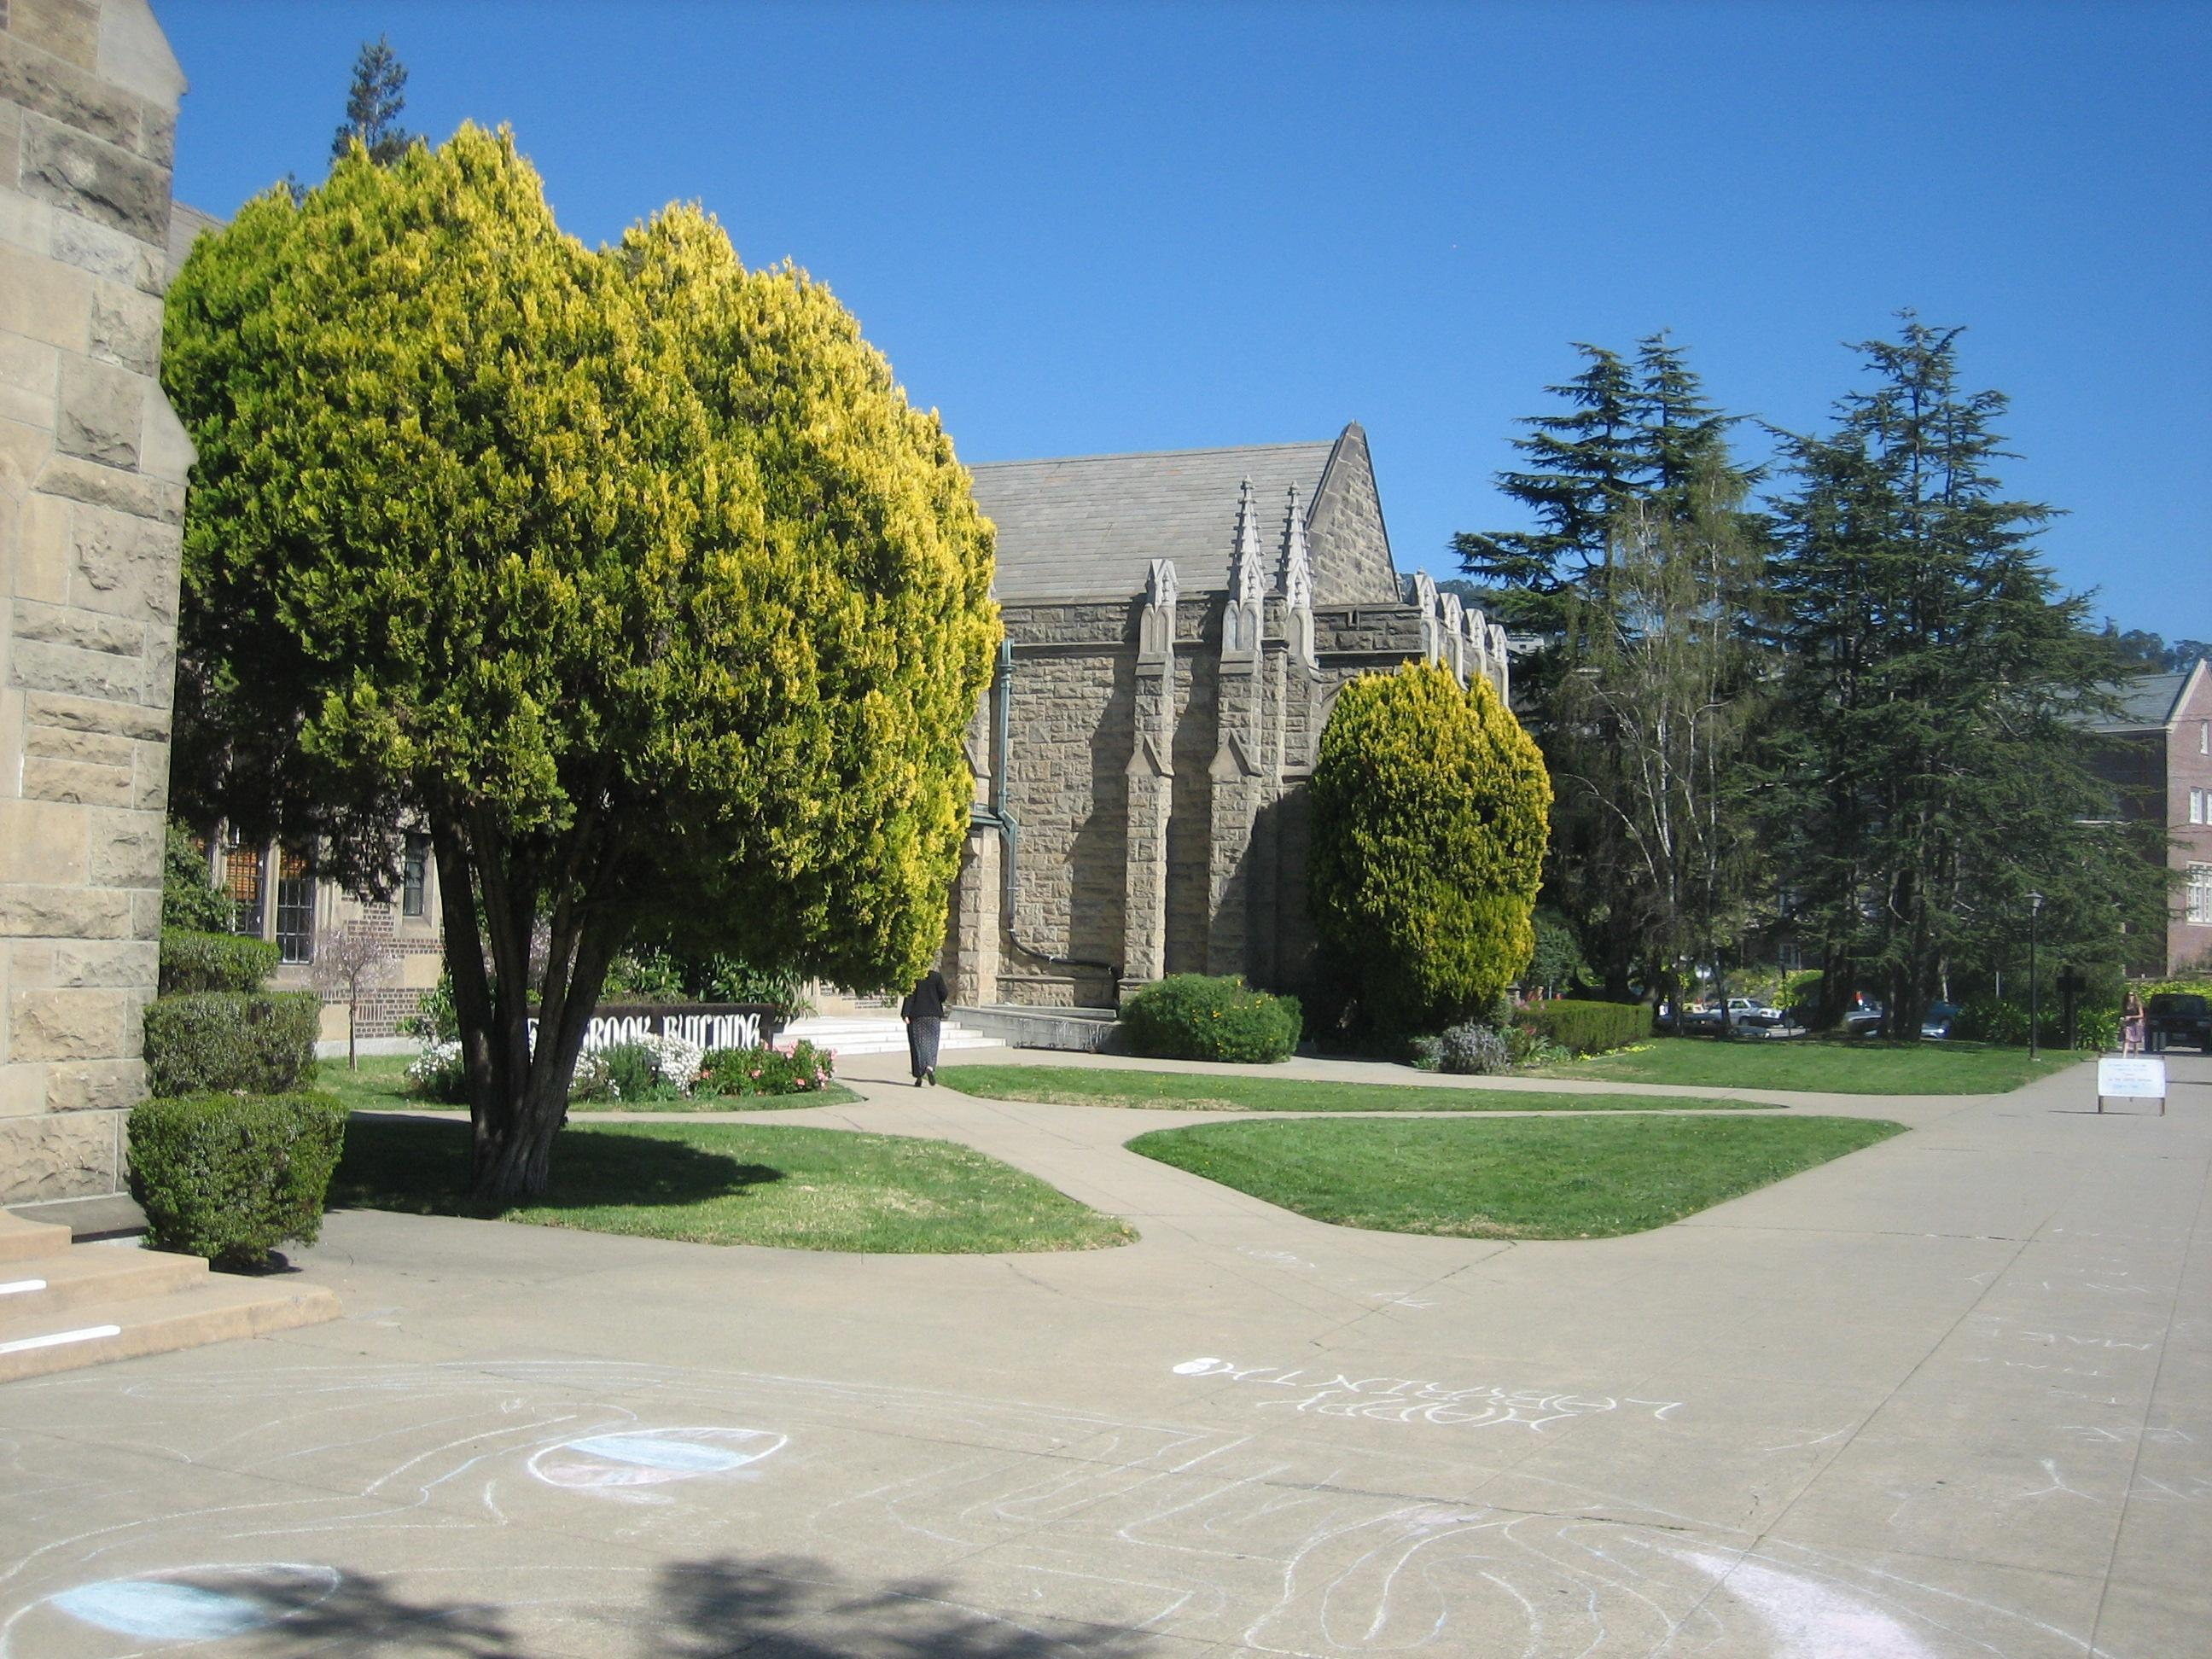
\includegraphics[width=10cm,height=10cm]{\input_image}};

\pic[shift={(0,0,0)}] at (0,0,0)
    {RightBandedBox={
        name=conv_0,
        caption=0,
        xlabel={(32,)},
        zlabel=I,
        fill=\ConvColor,
        bandfill=\ConvReluColor,
        height=40,
        depth=40,
        width={2}
        }
    };

\pic[shift={(3,0,0)}] at (conv_0-east)
    {RightBandedBox={
        name=conv_1,
        caption=1,
        xlabel={(64,)},
        zlabel=,
        fill=\ConvColor,
        bandfill=\ConvReluColor,
        height=20.0,
        depth=20.0,
        width={3.0}
        }
    };

\draw [connection] (conv_0-east) -- node {\midarrow} (conv_1-west);

\pic[shift={(0,0,0)}] at (conv_1-east)
    {RightBandedBox={
        name=conv_2,
        caption=2,
        xlabel={(32,)},
        zlabel=,
        fill=\ConvColor,
        bandfill=\ConvReluColor,
        height=20.0,
        depth=20.0,
        width={2.5}
        }
    };

\pic[shift={(0,0,0)}] at (conv_2-east)
    {RightBandedBox={
        name=conv_3,
        caption=3,
        xlabel={(64,)},
        zlabel=I/2,
        fill=\ConvColor,
        bandfill=\ConvReluColor,
        height=20.0,
        depth=20.0,
        width={3.0}
        }
    };

\draw[densely dashed]
    (conv_0-nearnortheast) coordinate(a) -- (conv_1-nearnorthwest)
    (conv_0-nearsoutheast) coordinate(b) -- (conv_1-nearsouthwest)
    (conv_0-farsoutheast) coordinate(c) -- (conv_1-farsouthwest)
    (conv_0-farnortheast) coordinate(d) -- (conv_1-farnorthwest)

    (a)--(b)--(c)--(d)
    ;

\pic[shift={(1.5,0,0)}] at (conv_3-east)
    {Box={
        name=short_4,
        caption=4,
        zlabel=,
        fill=\ShortcutColor,
        height=20.0,
        depth=20.0,
        width={1}
        }
    };

\path (conv_1-south) -- (conv_1-north) coordinate[pos=1.3] (conv_1-dummy) ;
\path (conv_1-dummy |- short_4-northwest) coordinate (short_4-dummy)  ;

\draw [connection] (conv_1-north)
-- node {}(conv_1-north |- conv_1-dummy)
-- node {\midarrow}(conv_1-dummy -| short_4-northwest)
-- node {}(short_4-northwest);

\pic[shift={(1,0,0)}] at (short_4-east)
    {RightBandedBox={
        name=conv_5,
        caption=5,
        xlabel={(128,)},
        zlabel=,
        fill=\ConvColor,
        bandfill=\ConvReluColor,
        height=10.0,
        depth=10.0,
        width={3.5}
        }
    };

\draw [connection] (short_4-east) -- node {\midarrow} (conv_5-west);

\pic[shift={(0,0,0)}] at (conv_5-east)
    {RightBandedBox={
        name=conv_6,
        caption=6,
        xlabel={(64,)},
        zlabel=,
        fill=\ConvColor,
        bandfill=\ConvReluColor,
        height=10.0,
        depth=10.0,
        width={3.0}
        }
    };

\pic[shift={(0,0,0)}] at (conv_6-east)
    {RightBandedBox={
        name=conv_7,
        caption=7,
        xlabel={(128,)},
        zlabel=,
        fill=\ConvColor,
        bandfill=\ConvReluColor,
        height=10.0,
        depth=10.0,
        width={3.5}
        }
    };

\draw[densely dashed]
    (short_4-nearnortheast) coordinate(a) -- (conv_5-nearnorthwest)
    (short_4-nearsoutheast) coordinate(b) -- (conv_5-nearsouthwest)
    (short_4-farsoutheast) coordinate(c) -- (conv_5-farsouthwest)
    (short_4-farnortheast) coordinate(d) -- (conv_5-farnorthwest)

    (a)--(b)--(c)--(d)
    ;

\pic[shift={(1,0,0)}] at (conv_7-east)
    {Box={
        name=short_8,
        caption=8,
        zlabel=I/4,
        fill=\ShortcutColor,
        height=10.0,
        depth=10.0,
        width={1}
        }
    };

\path (conv_5-south) -- (conv_5-north) coordinate[pos=1.5] (conv_5-dummy) ;
\path (conv_5-dummy |- short_8-north) coordinate (short_8-dummy)  ;

\draw [connection] (conv_5-north)
-- node {}(conv_5-north |- conv_5-dummy)
-- node {\midarrow}(conv_5-dummy -| short_8-north)
-- node {}(short_8-north);

\draw [connection] (conv_7-east) -- node {\midarrow} (short_8-west);

\pic[shift={(1,0,0)}] at (short_8-east)
    {Box={
        name=short_11,
        caption=11,
        zlabel=I/8,
        fill=\ShortcutColor,
        height=5.0,
        depth=5.0,
        width={1}
        }
    };

\draw [connection] (short_8-east) -- node [fill=white,inner sep=1pt, opacity=1] {\ldots} (short_11-west);

\pic[shift={(1,0,0)}] at (short_11-east)
    {Box={
        name=short_36,
        caption=36,
        zlabel=,
        fill=\ShortcutColor,
        height=2.5,
        depth=2.5,
        width={1}
        }
    };

\draw [connection] (short_11-east) -- node [fill=white,inner sep=1pt, opacity=1] {\ldots} (short_36-west);

\pic[shift={(1,0,0)}] at (short_36-east)
    {Box={
        name=short_61,
        caption=61,
        zlabel=,
        fill=\ShortcutColor,
        height=1.25,
        depth=1.25,
        width={1}
        }
    };

\draw [connection] (short_36-east) -- node [fill=white,inner sep=1pt, opacity=1] {\ldots} (short_61-west);

\pic[shift={(1,0,0)}] at (short_61-east)
    {RightBandedBox={
        name=conv_79,
        caption=79,
        xlabel={(512,)},
        zlabel=,
        fill=\ConvColor,
        bandfill=\ConvReluColor,
        height=1.25,
        depth=1.25,
        width={4.5}
        }
    };

\draw [connection] (short_61-east) -- node [fill=white,inner sep=1pt, opacity=1] {\ldots} (conv_79-west);

\pic[shift={(-1.3333333333333333,0,3)}] at (conv_79-east)
    {RightBandedBox={
        name=conv_80,
        caption= ,
        xlabel={((),)},
        zlabel=,
        fill=\ConvColor,
        bandfill=\ConvReluColor,
        height=1.25,
        depth=1.25,
        width={4.5}
        }
    };

\draw [connection] (conv_79-near) -- node {\midarrow} (conv_80-far);

\pic[shift={(-1.3333333333333333,0,3)}] at (conv_80-east)
    {RightBandedBox={
        name=conv_81,
        caption= ,
        xlabel={((),)},
        zlabel=,
        fill=\ConvColor,
        bandfill=\ConvReluColor,
        height=1.25,
        depth=1.25,
        width={5.0}
        }
    };

\draw [connection] (conv_80-near) -- node {\midarrow} (conv_81-far);

\pic[shift={(-1.3333333333333333,0,3)}] at (conv_81-east)
    {RightBandedBox={
        name=conv_82,
        caption=82,
        xlabel={(256,)},
        zlabel=I/32,
        fill=\ConvColor,
        bandfill=\ConvReluColor,
        height=1.25,
        depth=1.25,
        width={4.0}
        }
    };

\draw [connection] (conv_81-near) -- node {\midarrow} (conv_82-far);

\pic[shift={(-0.75, 0, 3)}] at (conv_82-east)
    {Box={
        name=yolo_83,
        caption=83,
        zlabel=,
        fill=\DetectColor,
        height=1.25,
        depth=1.25,
        width={1}
        }
    };

\node[canvas is zy plane at x=0] (image_yolo_83) at (yolo_83-east) {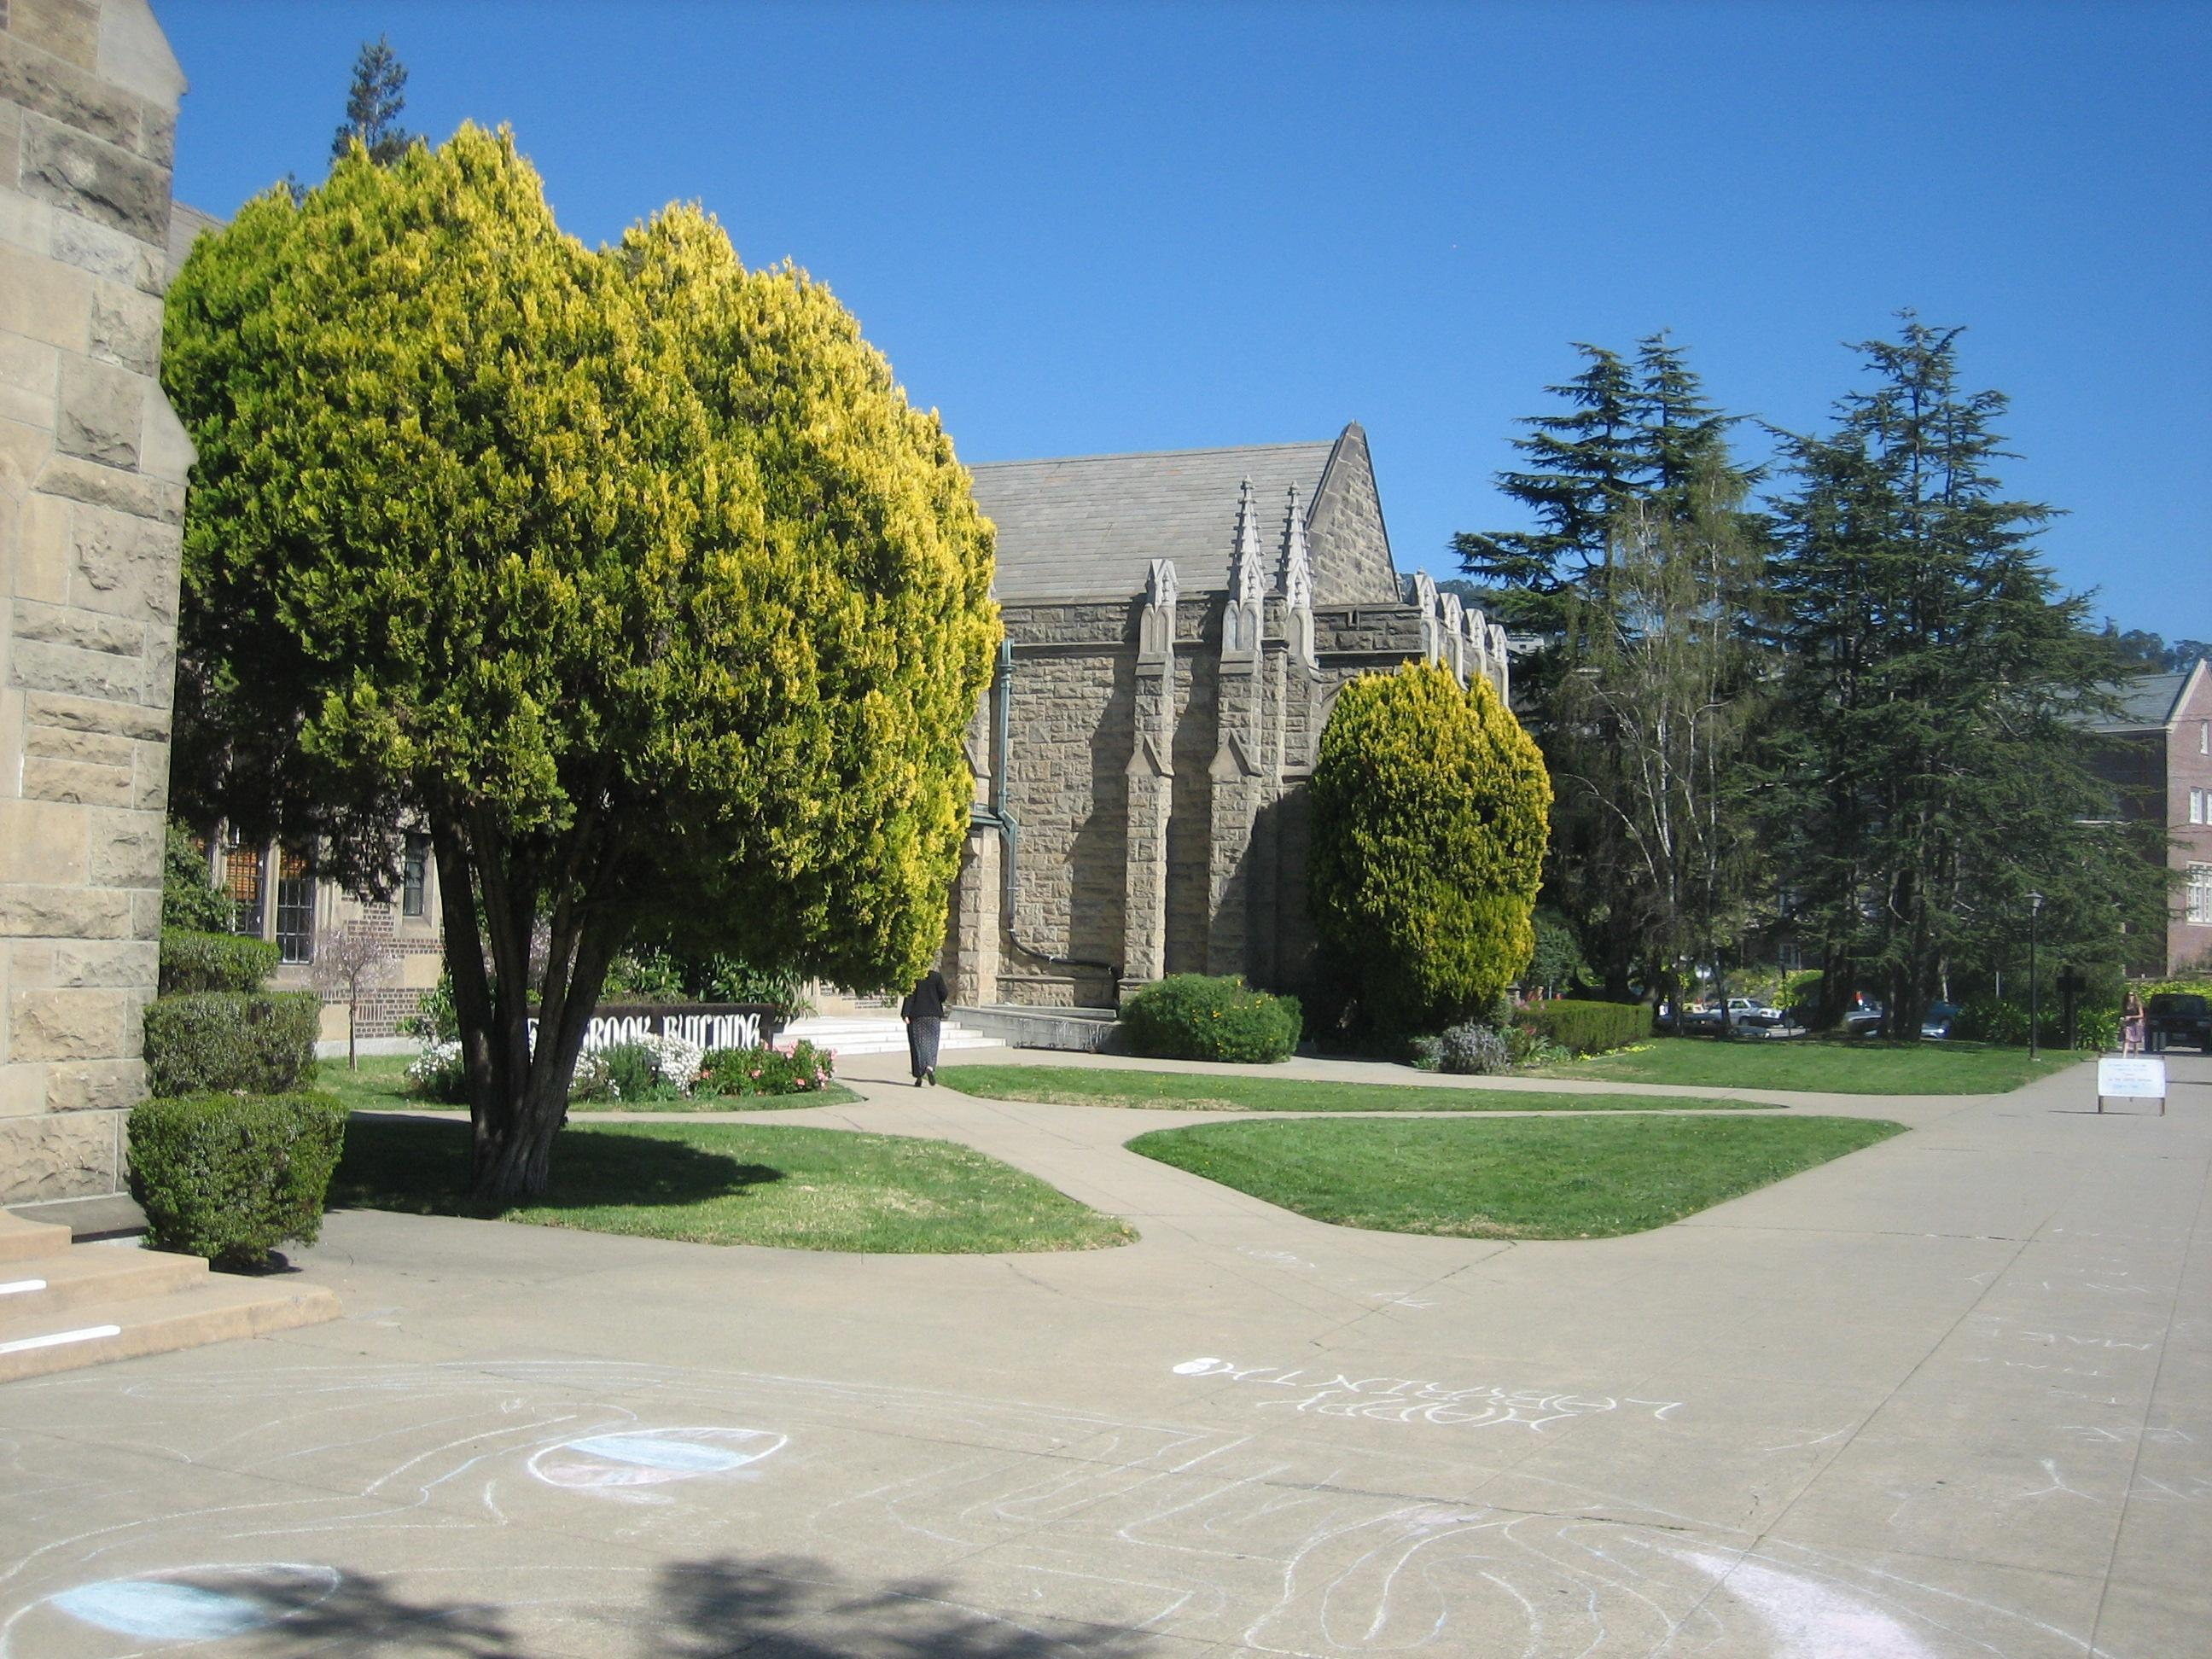
\includegraphics[width=0.25cm,height=0.25cm]{\input_image}};

\node[canvas is zy plane at x=0] (grid_yolo_83) at (image_yolo_83) {\drawgrid{0.25}{0.25}{0.25}};

\draw [connection] (conv_82-near) -- node {\midarrow} (yolo_83-far);

\pic[shift={(1,0,0)}] at (conv_79-east)
    {RightBandedBox={
        name=conv_85,
        caption=85,
        xlabel={(256,)},
        zlabel=,
        fill=\ConvColor,
        bandfill=\ConvReluColor,
        height=1.25,
        depth=1.25,
        width={4.0}
        }
    };

\draw [connection] (conv_79-east) -- node {\midarrow} (conv_85-west);

\pic[shift={(1,0,0)}] at (conv_85-east)
    {Box={
        name=conv_86_0,
        fill=\UpsampleColor,
        height=1.25,
        depth=1.25,
        width={1}
        }
    };
\pic[shift={(1,0,0)}] at (conv_86_0-east)
    {Box={
        name=conv_86,
        fill=\UpsampleColor,
        height=2.5,
        depth=2.5,
        width={1}
        }
    };
\draw[densely dashed]
    (conv_86_0-nearnortheast) coordinate(a) -- (conv_86-nearnorthwest)
    (conv_86_0-nearsoutheast) coordinate(b) -- (conv_86-nearsouthwest)
    (conv_86_0-farsoutheast) coordinate(c) -- (conv_86-farsouthwest)
    (conv_86_0-farnortheast) coordinate(d) -- (conv_86-farnorthwest)

    (a)--(b)--(c)--(d)
    ;

\draw [connection] (conv_85-east) -- node {\midarrow} (conv_86_0-west);

\pic[shift={(1.25,0,0)}] at (conv_86-east)
    {Ball={
        name=conc_87,
        caption=,
        fill=\ConcColor,
        opacity=0.5,
        radius=2,
        logo=$\oplus$
        }
    };

\draw [connection] (conv_86-east) -- node {\midarrow} (conc_87-west);

\path (short_61-south) -- (short_61-north) coordinate[pos=3] (short_61-dummy) ;
\path (short_61-dummy |- conc_87-north) coordinate (conc_87-dummy)  ;

\draw [connection] (short_61-north)
-- node {}(short_61-north |- short_61-dummy)
-- node {\midarrow}(short_61-dummy -| conc_87-north)
-- node {}(conc_87-north);

\pic[shift={(1,0,0)}] at (conc_87-east)
    {RightBandedBox={
        name=conv_90,
        caption=90,
        xlabel={(512,)},
        zlabel=,
        fill=\ConvColor,
        bandfill=\ConvReluColor,
        height=2.5,
        depth=2.5,
        width={4.5}
        }
    };

\draw [connection] (conc_87-east) -- node [fill=white,inner sep=1pt, opacity=1] {\ldots} (conv_90-west);

\pic[shift={(-1.3333333333333333,0,3)}] at (conv_90-east)
    {RightBandedBox={
        name=conv_91,
        caption= ,
        xlabel={((),)},
        zlabel=,
        fill=\ConvColor,
        bandfill=\ConvReluColor,
        height=2.5,
        depth=2.5,
        width={4.0}
        }
    };

\draw [connection] (conv_90-near) -- node {\midarrow} (conv_91-far);

\pic[shift={(-1.3333333333333333,0,3)}] at (conv_91-east)
    {RightBandedBox={
        name=conv_92,
        caption= ,
        xlabel={((),)},
        zlabel=,
        fill=\ConvColor,
        bandfill=\ConvReluColor,
        height=2.5,
        depth=2.5,
        width={4.5}
        }
    };

\draw [connection] (conv_91-near) -- node {\midarrow} (conv_92-far);

\pic[shift={(-1.3333333333333333,0,3)}] at (conv_92-east)
    {RightBandedBox={
        name=conv_93,
        caption=93,
        xlabel={(256,)},
        zlabel=I/16,
        fill=\ConvColor,
        bandfill=\ConvReluColor,
        height=2.5,
        depth=2.5,
        width={4.0}
        }
    };

\draw [connection] (conv_92-near) -- node {\midarrow} (conv_93-far);

\pic[shift={(-0.75, 0, 3)}] at (conv_93-east)
    {Box={
        name=yolo_94,
        caption=94,
        zlabel=,
        fill=\DetectColor,
        height=2.5,
        depth=2.5,
        width={1}
        }
    };

\node[canvas is zy plane at x=0] (image_yolo_94) at (yolo_94-east) {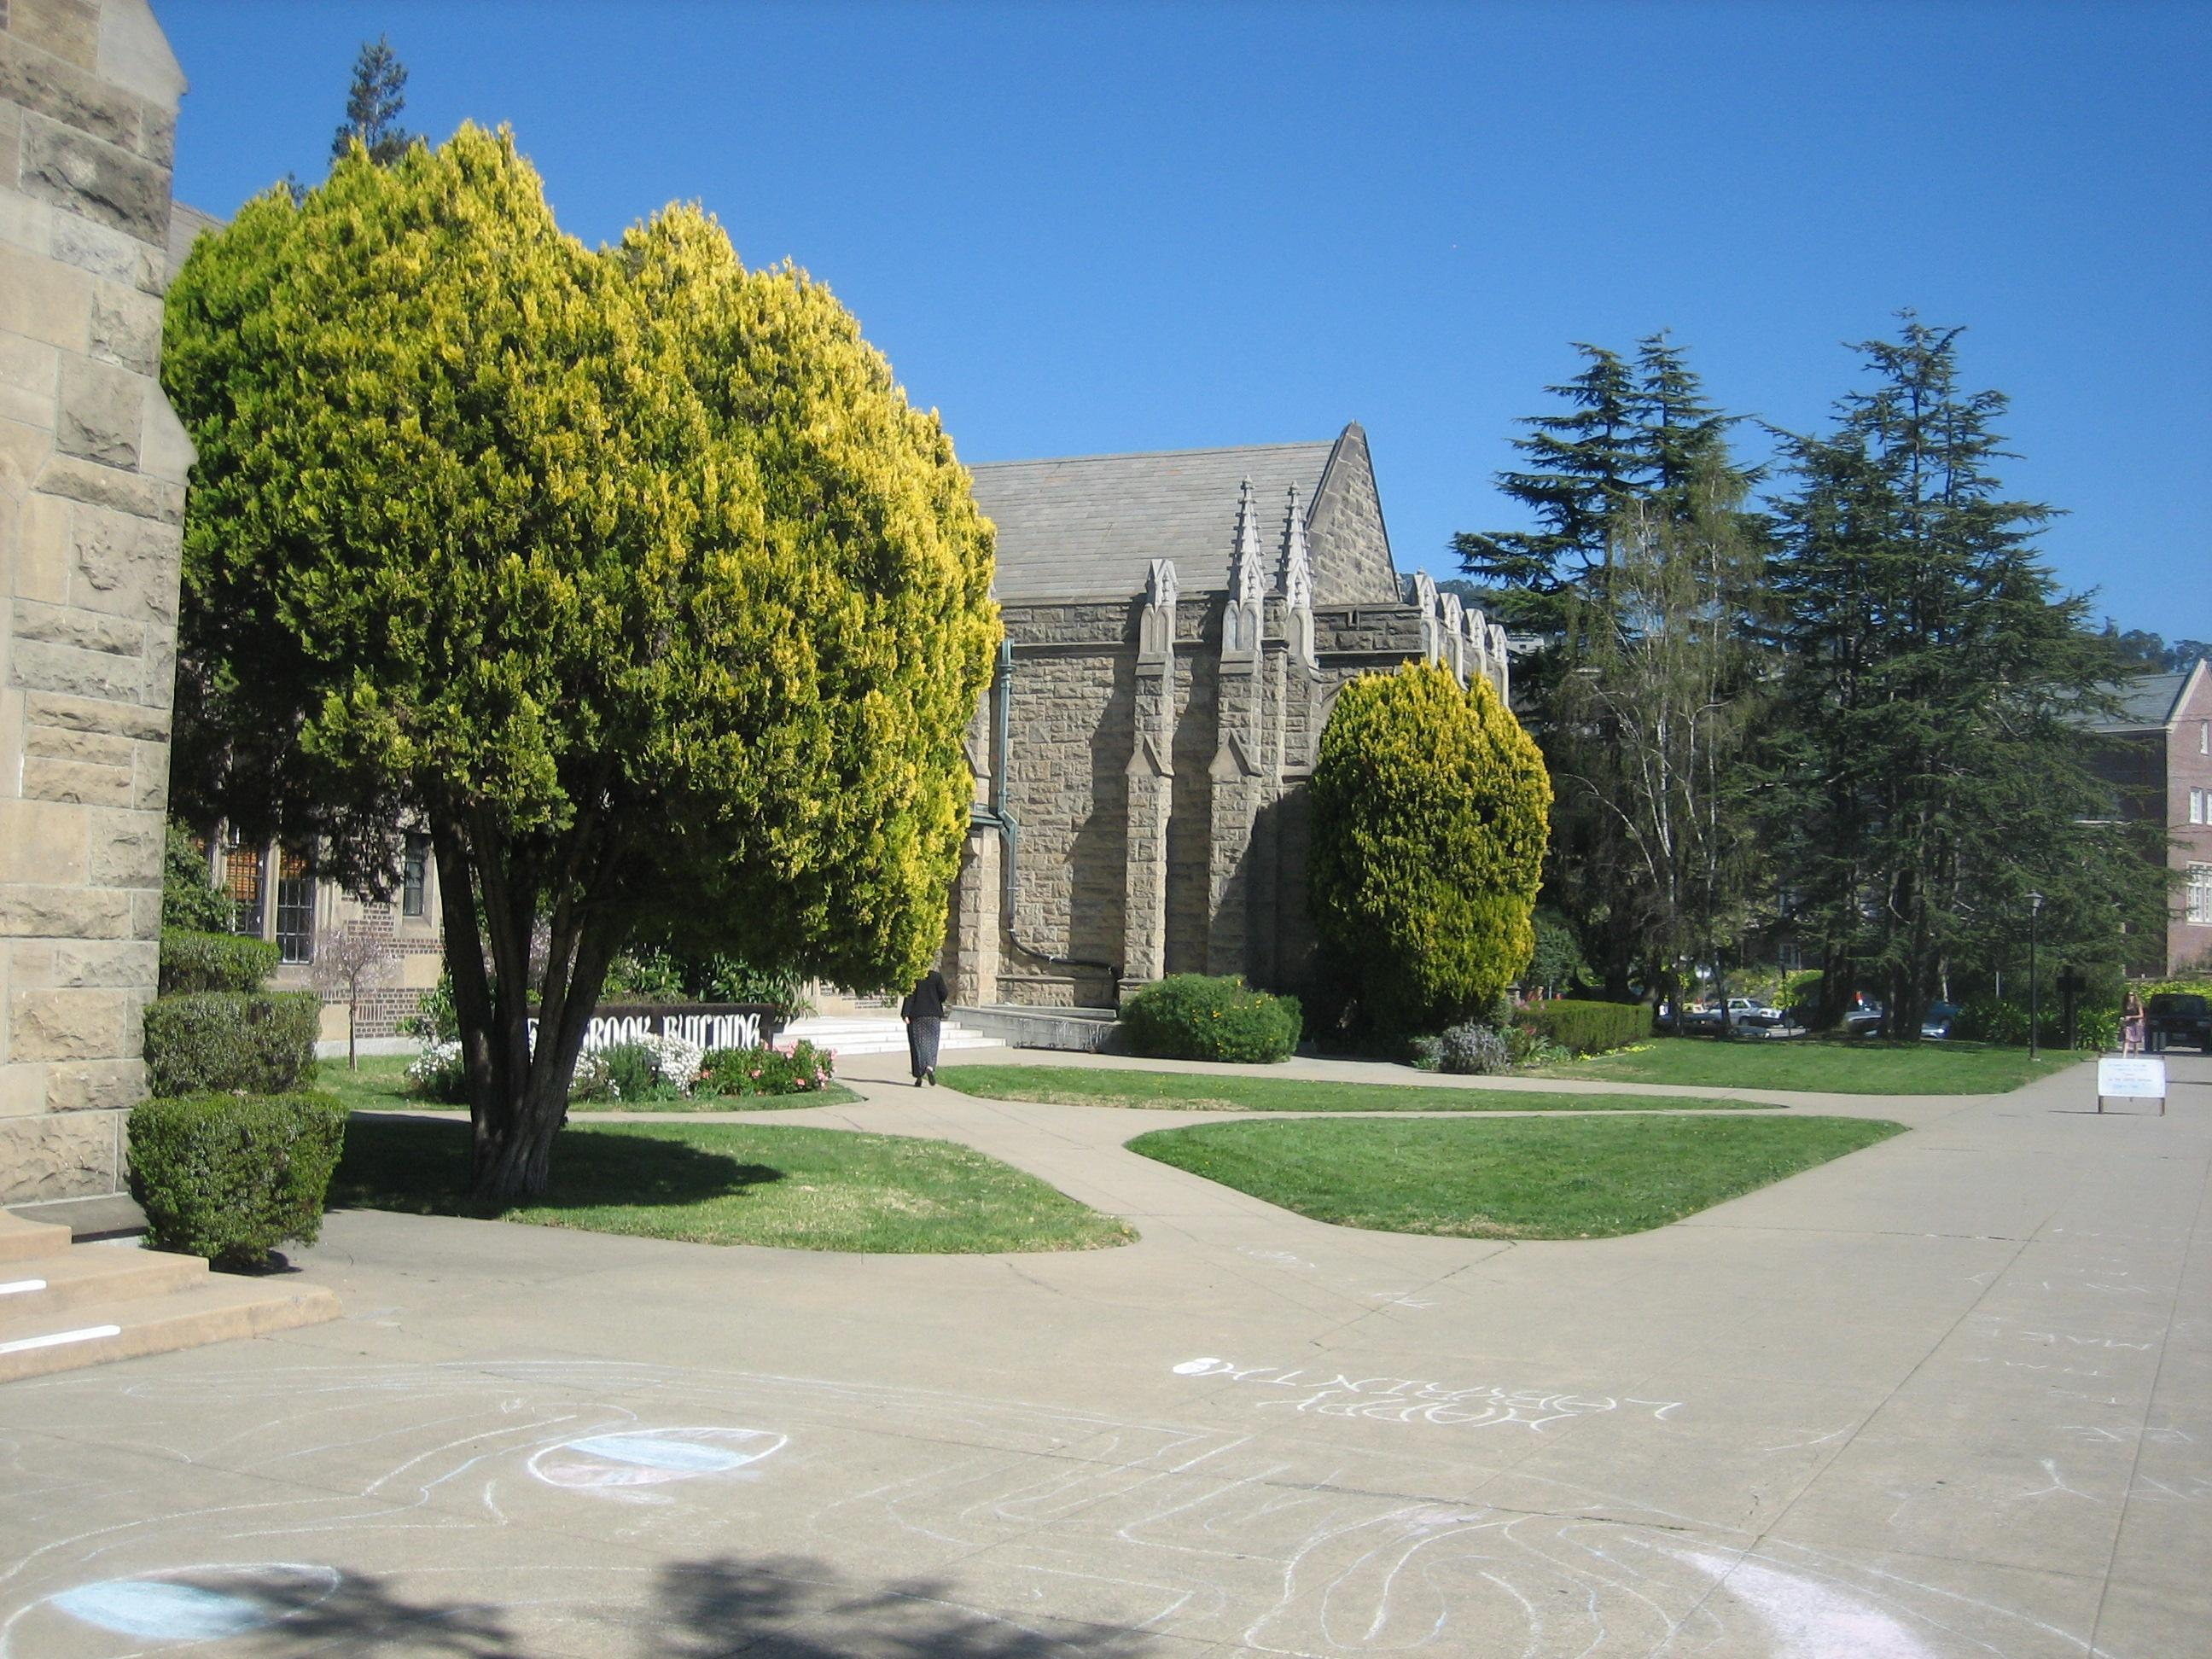
\includegraphics[width=0.5cm,height=0.5cm]{\input_image}};

\node[canvas is zy plane at x=0] (grid_yolo_94) at (image_yolo_94) {\drawgrid{0.5}{0.5}{0.5}};

\draw [connection] (conv_93-near) -- node {\midarrow} (yolo_94-far);

\pic[shift={(1,0,0)}] at (conv_90-east)
    {RightBandedBox={
        name=conv_96,
        caption=96,
        xlabel={(128,)},
        zlabel=,
        fill=\ConvColor,
        bandfill=\ConvReluColor,
        height=2.5,
        depth=2.5,
        width={3.5}
        }
    };

\draw [connection] (conv_90-east) -- node {\midarrow} (conv_96-west);

\pic[shift={(1,0,0)}] at (conv_96-east)
    {Box={
        name=conv_97_0,
        fill=\UpsampleColor,
        height=2.5,
        depth=2.5,
        width={1}
        }
    };
\pic[shift={(1,0,0)}] at (conv_97_0-east)
    {Box={
        name=conv_97,
        fill=\UpsampleColor,
        height=5.0,
        depth=5.0,
        width={1}
        }
    };
\draw[densely dashed]
    (conv_97_0-nearnortheast) coordinate(a) -- (conv_97-nearnorthwest)
    (conv_97_0-nearsoutheast) coordinate(b) -- (conv_97-nearsouthwest)
    (conv_97_0-farsoutheast) coordinate(c) -- (conv_97-farsouthwest)
    (conv_97_0-farnortheast) coordinate(d) -- (conv_97-farnorthwest)

    (a)--(b)--(c)--(d)
    ;

\draw [connection] (conv_96-east) -- node {\midarrow} (conv_97_0-west);

\pic[shift={(1.25,0,0)}] at (conv_97-east)
    {Ball={
        name=conc_98,
        caption=,
        fill=\ConcColor,
        opacity=0.5,
        radius=2,
        logo=$\oplus$
        }
    };

\draw [connection] (conv_97-east) -- node {\midarrow} (conc_98-west);

\path (short_36-south) -- (short_36-north) coordinate[pos=3.25] (short_36-dummy) ;
\path (short_36-dummy |- conc_98-north) coordinate (conc_98-dummy)  ;

\draw [connection] (short_36-north)
-- node {}(short_36-north |- short_36-dummy)
-- node {\midarrow}(short_36-dummy -| conc_98-north)
-- node {}(conc_98-north);

\pic[shift={(1,0,0)}] at (conc_98-east)
    {RightBandedBox={
        name=conv_102,
        caption=103,
        xlabel={(512,)},
        zlabel=,
        fill=\ConvColor,
        bandfill=\ConvReluColor,
        height=5.0,
        depth=5.0,
        width={4.5}
        }
    };

\draw [connection] (conc_98-east) -- node [fill=white,inner sep=1pt, opacity=1] {\ldots} (conv_102-west);

\pic[shift={(-1.0,0,4)}] at (conv_102-east)
    {RightBandedBox={
        name=conv_103,
        caption= ,
        xlabel={((),)},
        zlabel=,
        fill=\ConvColor,
        bandfill=\ConvReluColor,
        height=5.0,
        depth=5.0,
        width={3.5}
        }
    };

\draw [connection] (conv_102-near) -- node {\midarrow} (conv_103-far);

\pic[shift={(-1.0,0,4)}] at (conv_103-east)
    {RightBandedBox={
        name=conv_104,
        caption= ,
        xlabel={((),)},
        zlabel=,
        fill=\ConvColor,
        bandfill=\ConvReluColor,
        height=5.0,
        depth=5.0,
        width={4.0}
        }
    };

\draw [connection] (conv_103-near) -- node {\midarrow} (conv_104-far);

\pic[shift={(-1.0,0,4)}] at (conv_104-east)
    {RightBandedBox={
        name=conv_105,
        caption=105,
        xlabel={(256,)},
        zlabel=I/8,
        fill=\ConvColor,
        bandfill=\ConvReluColor,
        height=5.0,
        depth=5.0,
        width={4.0}
        }
    };

\draw [connection] (conv_104-near) -- node {\midarrow} (conv_105-far);

\pic[shift={(-1, 0, 4)}] at (conv_105-east)
    {Box={
        name=yolo_106,
        caption=106,
        zlabel=,
        fill=\DetectColor,
        height=5.0,
        depth=5.0,
        width={1}
        }
    };

\node[canvas is zy plane at x=0] (image_yolo_106) at (yolo_106-east) {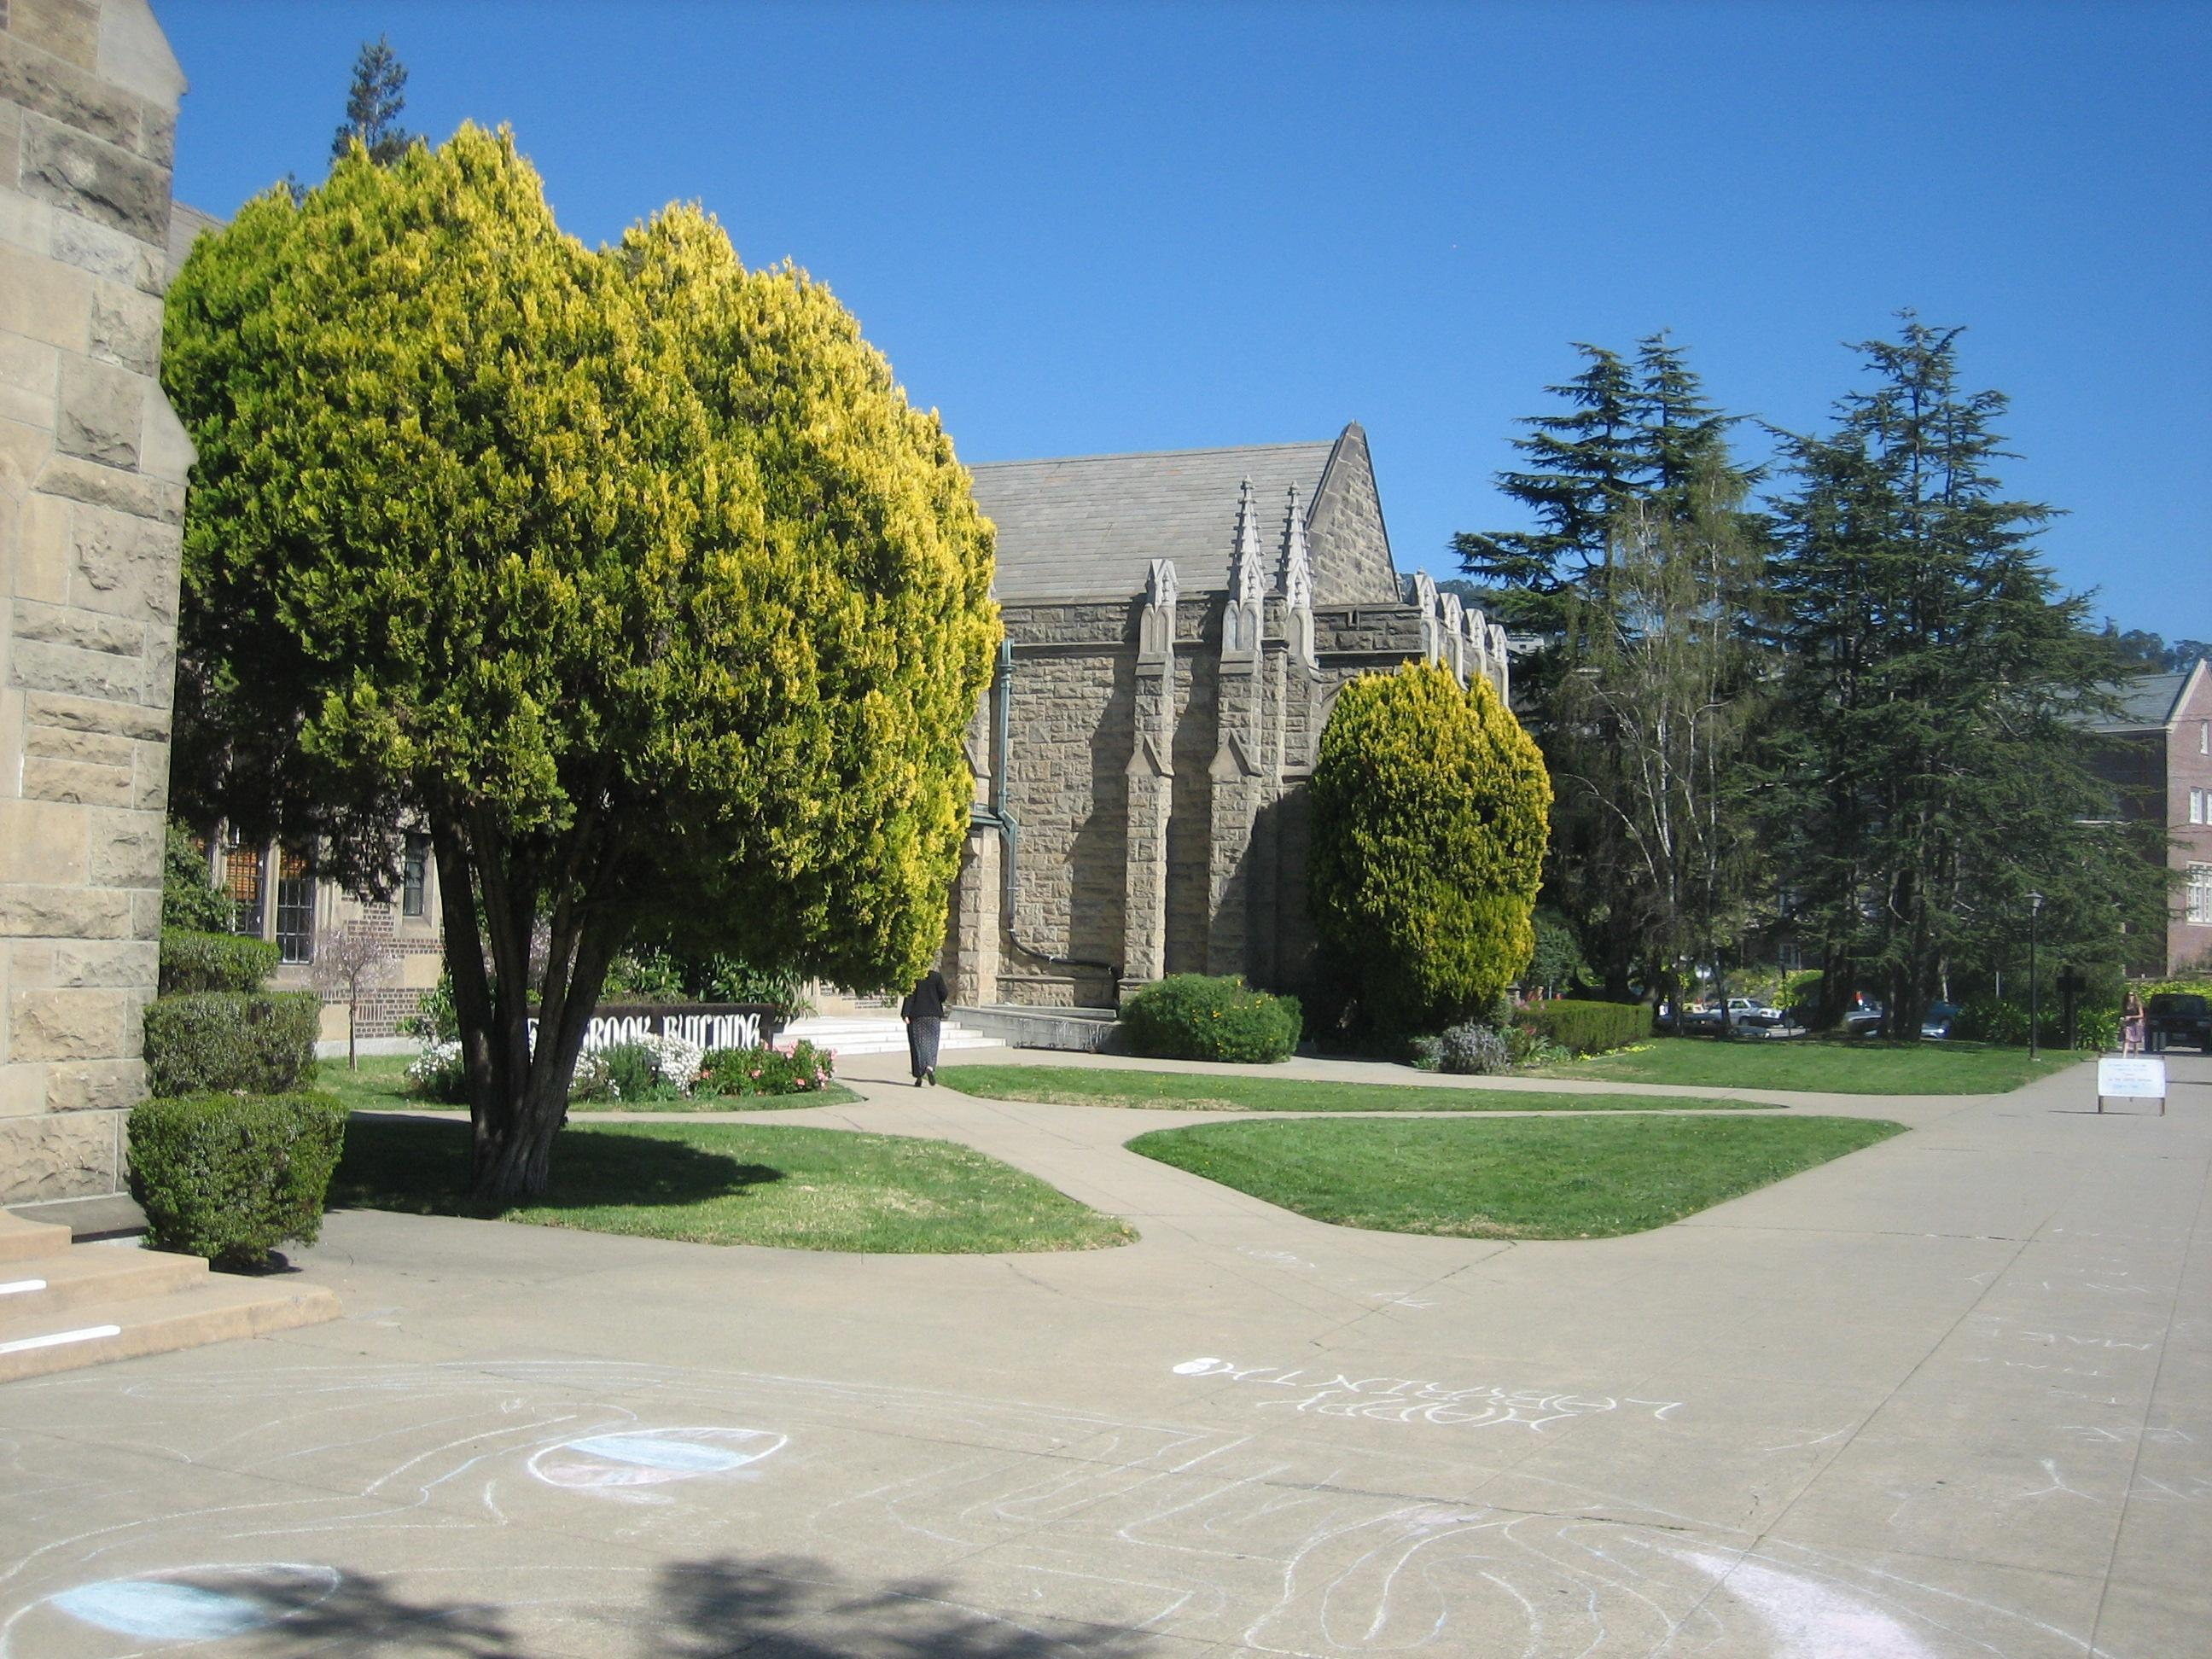
\includegraphics[width=1.0cm,height=1.0cm]{\input_image}};

\node[canvas is zy plane at x=0] (grid_yolo_106) at (image_yolo_106) {\drawgrid{1.0}{1.0}{1.0}};

\draw [connection] (conv_105-near) -- node {\midarrow} (yolo_106-far);

\pic[shift={(1,0,0)}] at (conv_102-east)
    {RightBandedBox={
        name=conv_108,
        caption=108,
        xlabel={(128,)},
        zlabel=,
        fill=\ConvColor,
        bandfill=\ConvReluColor,
        height=5.0,
        depth=5.0,
        width={3.5}
        }
    };

\draw [connection] (conv_102-east) -- node {\midarrow} (conv_108-west);

\pic[shift={(1,0,0)}] at (conv_108-east)
    {Box={
        name=conv_109_0,
        fill=\UpsampleColor,
        height=5.0,
        depth=5.0,
        width={1}
        }
    };
\pic[shift={(1,0,0)}] at (conv_109_0-east)
    {Box={
        name=conv_109,
        fill=\UpsampleColor,
        height=10.0,
        depth=10.0,
        width={1}
        }
    };
\draw[densely dashed]
    (conv_109_0-nearnortheast) coordinate(a) -- (conv_109-nearnorthwest)
    (conv_109_0-nearsoutheast) coordinate(b) -- (conv_109-nearsouthwest)
    (conv_109_0-farsoutheast) coordinate(c) -- (conv_109-farsouthwest)
    (conv_109_0-farnortheast) coordinate(d) -- (conv_109-farnorthwest)

    (a)--(b)--(c)--(d)
    ;

\draw [connection] (conv_108-east) -- node {\midarrow} (conv_109_0-west);

\pic[shift={(1.25,0,0)}] at (conv_109-east)
    {Ball={
        name=conc_110,
        caption=,
        fill=\ConcColor,
        opacity=0.5,
        radius=2,
        logo=$\oplus$
        }
    };

\draw [connection] (conv_109-east) -- node {\midarrow} (conc_110-west);

\path (short_11-south) -- (short_11-north) coordinate[pos=3] (short_11-dummy) ;
\path (short_11-dummy |- conc_110-north) coordinate (conc_110-dummy)  ;

\draw [connection] (short_11-north)
-- node {}(short_11-north |- short_11-dummy)
-- node {\midarrow}(short_11-dummy -| conc_110-north)
-- node {}(conc_110-north);

\pic[shift={(1,0,0)}] at (conc_110-east)
    {RightBandedBox={
        name=conv_114,
        caption=114,
        xlabel={(512,)},
        zlabel=,
        fill=\ConvColor,
        bandfill=\ConvReluColor,
        height=10.0,
        depth=10.0,
        width={4.5}
        }
    };

\draw [connection] (conc_110-east) -- node [fill=white,inner sep=1pt, opacity=1] {\ldots} (conv_114-west);

\pic[shift={(-0.6666666666666666,0,6)}] at (conv_114-east)
    {RightBandedBox={
        name=conv_115,
        caption= ,
        xlabel={((),)},
        zlabel=,
        fill=\ConvColor,
        bandfill=\ConvReluColor,
        height=10.0,
        depth=10.0,
        width={3.0}
        }
    };

\draw [connection] (conv_114-near) -- node {\midarrow} (conv_115-far);

\pic[shift={(-0.6666666666666666,0,6)}] at (conv_115-east)
    {RightBandedBox={
        name=conv_116,
        caption= ,
        xlabel={((),)},
        zlabel=,
        fill=\ConvColor,
        bandfill=\ConvReluColor,
        height=10.0,
        depth=10.0,
        width={3.5}
        }
    };

\draw [connection] (conv_115-near) -- node {\midarrow} (conv_116-far);

\pic[shift={(-0.6666666666666666,0,6)}] at (conv_116-east)
    {RightBandedBox={
        name=conv_117,
        caption=117,
        xlabel={(256,)},
        zlabel=I/4,
        fill=\ConvColor,
        bandfill=\ConvReluColor,
        height=10.0,
        depth=10.0,
        width={4.0}
        }
    };

\draw [connection] (conv_116-near) -- node {\midarrow} (conv_117-far);

\pic[shift={(-0.75, 0, 6)}] at (conv_117-east)
    {Box={
        name=yolo_4,
        caption=118,
        zlabel=,
        fill=\DetectColor,
        height=10.0,
        depth=10.0,
        width={1}
        }
    };

\node[canvas is zy plane at x=0] (image_yolo_4) at (yolo_4-east) {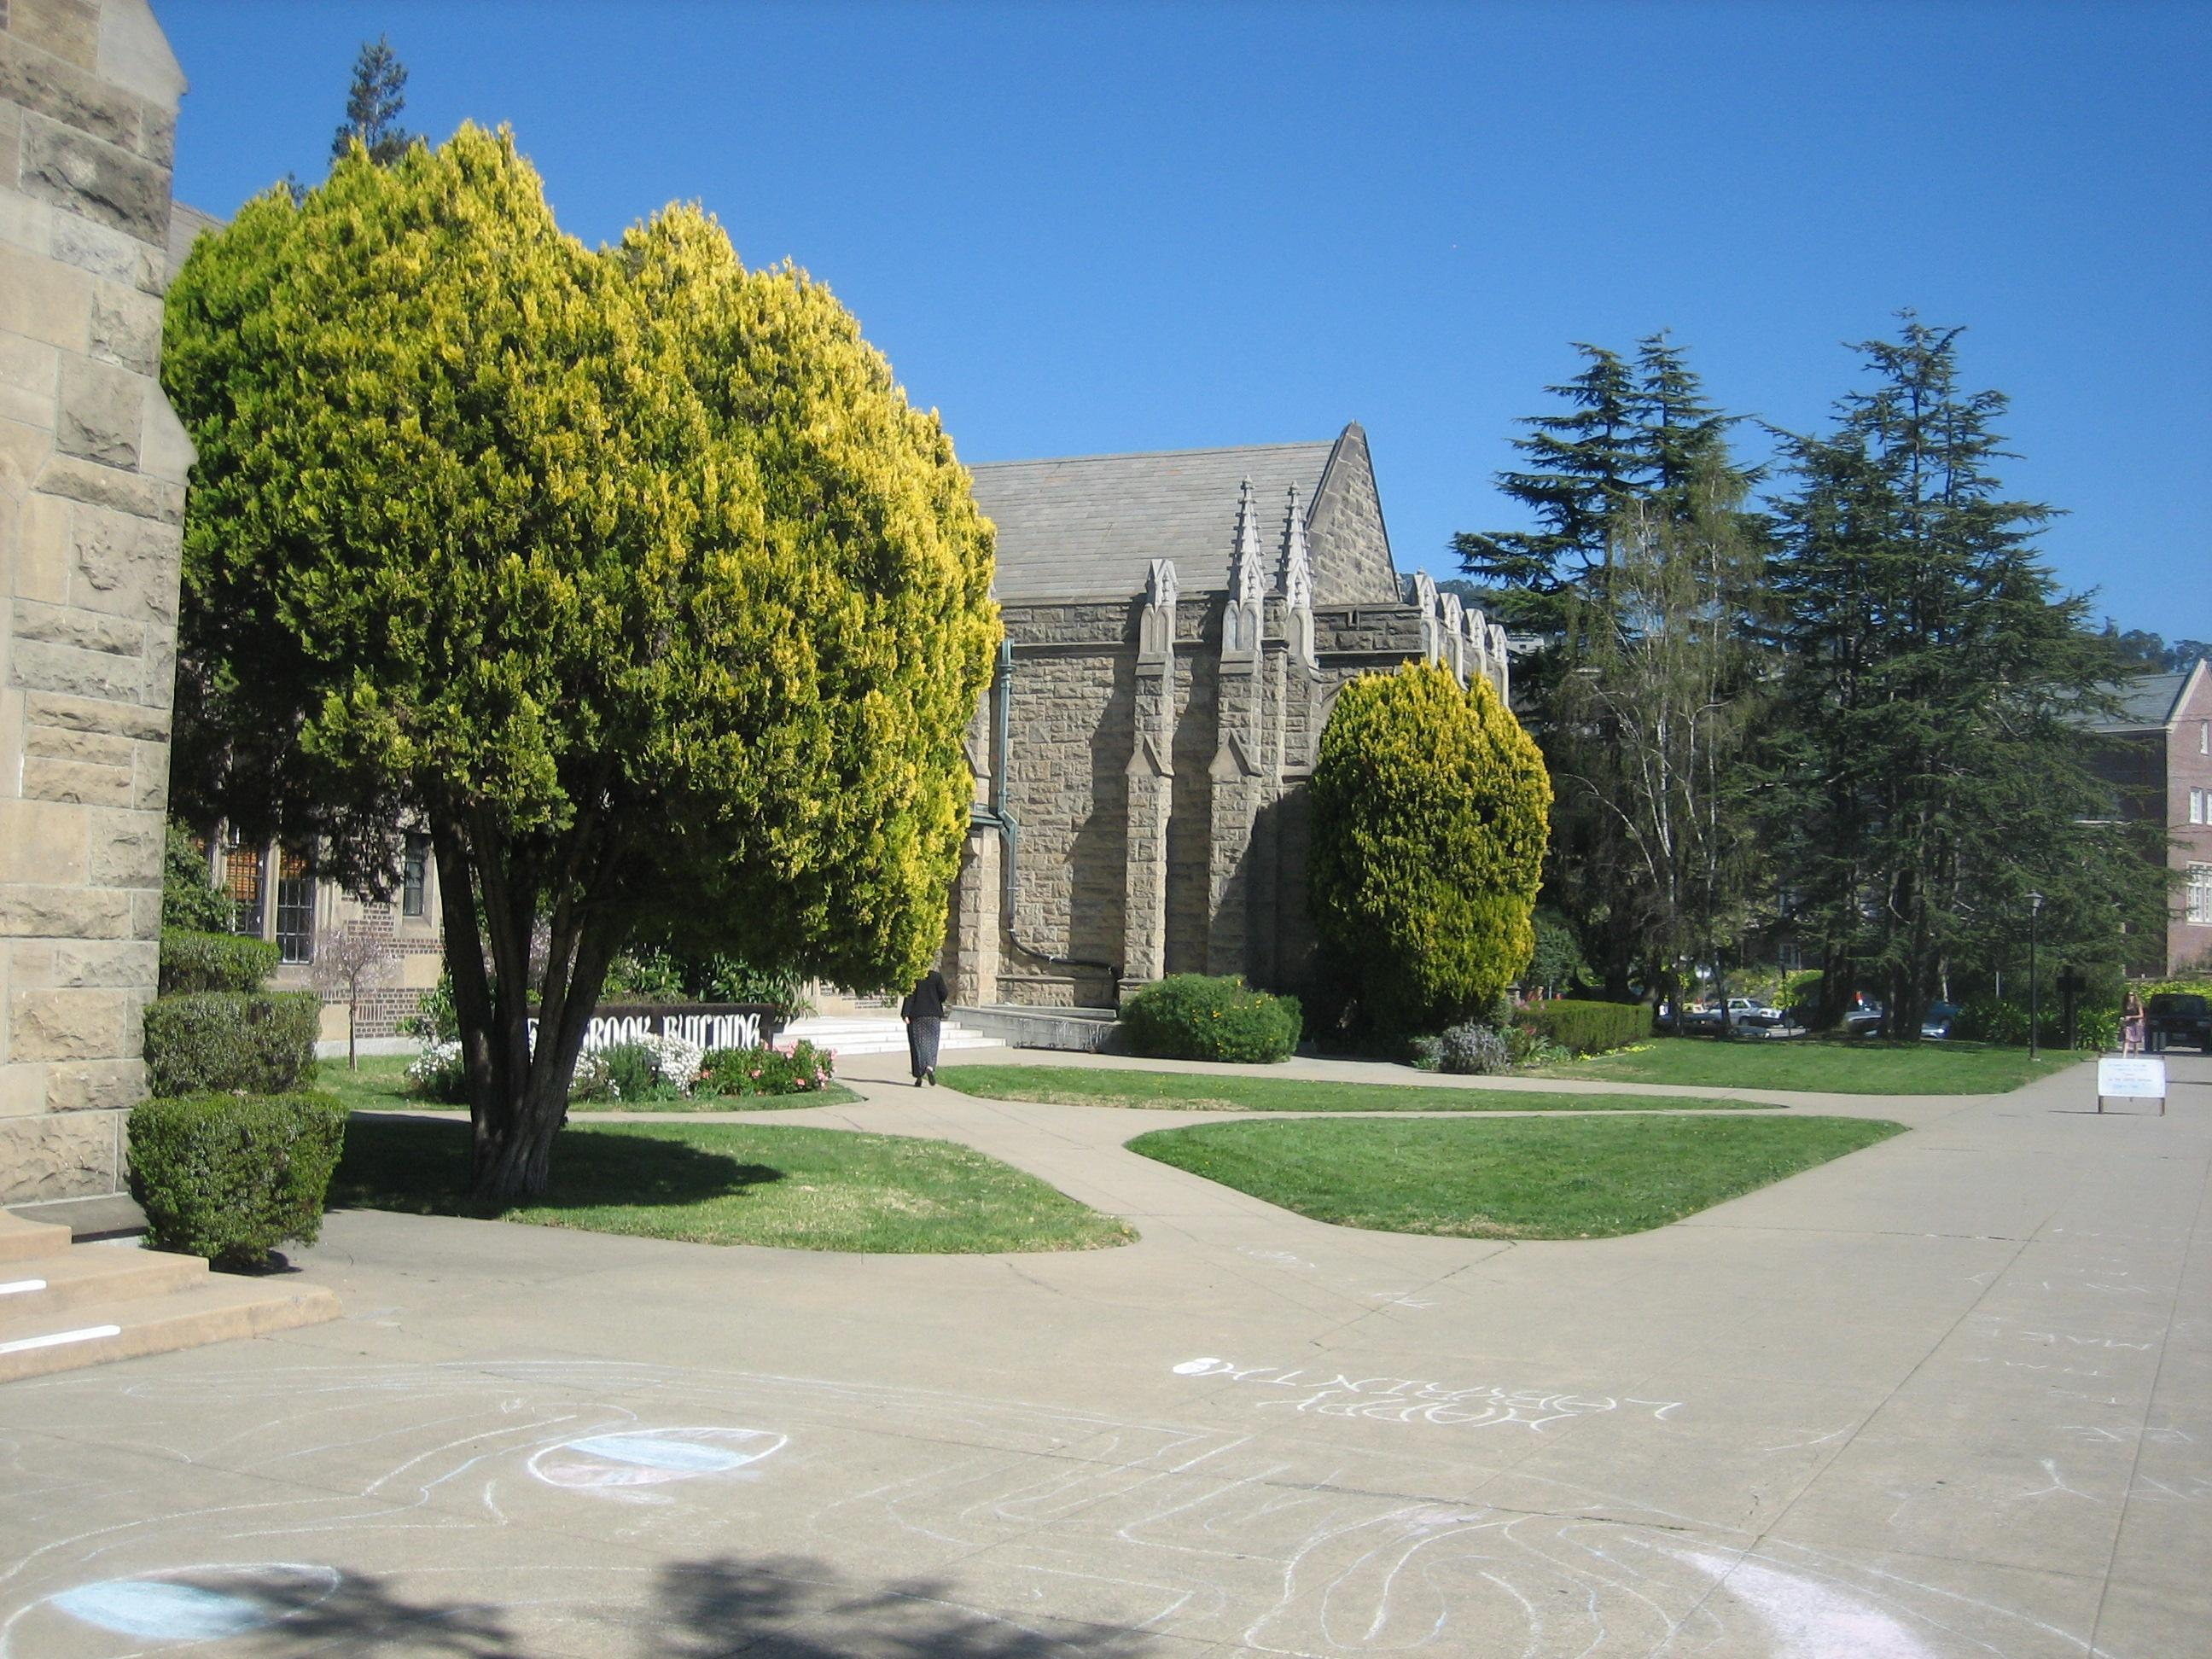
\includegraphics[width=2.0cm,height=2.0cm]{\input_image}};

\node[canvas is zy plane at x=0] (grid_yolo_4) at (image_yolo_4) {\drawgrid{2.0}{2.0}{0.15384615384615385}};

\draw [connection] (conv_117-near) -- node {\midarrow} (yolo_4-far);

\pic[shift={(1,0,0)}] at (conv_114-east)
    {RightBandedBox={
        name=conv_120,
        caption=120,
        xlabel={(128,)},
        zlabel=,
        fill=\ConvColor,
        bandfill=\ConvReluColor,
        height=10.0,
        depth=10.0,
        width={3.5}
        }
    };

\draw [connection] (conv_114-east) -- node {\midarrow} (conv_120-west);

\pic[shift={(1,0,0)}] at (conv_120-east)
    {Box={
        name=conv_121_0,
        fill=\UpsampleColor,
        height=10.0,
        depth=10.0,
        width={1}
        }
    };
\pic[shift={(1,0,0)}] at (conv_121_0-east)
    {Box={
        name=conv_121,
        fill=\UpsampleColor,
        height=20.0,
        depth=20.0,
        width={1}
        }
    };
\draw[densely dashed]
    (conv_121_0-nearnortheast) coordinate(a) -- (conv_121-nearnorthwest)
    (conv_121_0-nearsoutheast) coordinate(b) -- (conv_121-nearsouthwest)
    (conv_121_0-farsoutheast) coordinate(c) -- (conv_121-farsouthwest)
    (conv_121_0-farnortheast) coordinate(d) -- (conv_121-farnorthwest)

    (a)--(b)--(c)--(d)
    ;

\draw [connection] (conv_120-east) -- node {\midarrow} (conv_121_0-west);

\pic[shift={(1.5,0,0)}] at (conv_121-east)
    {Ball={
        name=conc_122,
        caption=,
        fill=\ConcColor,
        opacity=0.5,
        radius=2,
        logo=$\oplus$
        }
    };

\draw [connection] (conv_121-east) -- node {\midarrow} (conc_122-west);

\path (short_4-southeast) -- (short_4-northeast) coordinate[pos=1.5] (short_4-dummy) ;
\path (short_4-dummy |- conc_122-north) coordinate (conc_122-dummy)  ;

\draw [connection] (short_4-northeast)
-- node {}(short_4-northeast |- short_4-dummy)
-- node {\midarrow}(short_4-dummy -| conc_122-north)
-- node {}(conc_122-north);

\pic[shift={(1.5,0,0)}] at (conc_122-east)
    {RightBandedBox={
        name=conv_126,
        caption=126,
        xlabel={(128,)},
        zlabel=,
        fill=\ConvColor,
        bandfill=\ConvReluColor,
        height=20.0,
        depth=20.0,
        width={3.5}
        }
    };

\draw [connection] (conc_122-east) -- node [fill=white,inner sep=1pt, opacity=1] {\ldots} (conv_126-west);

\pic[shift={(-0.5,0,8)}] at (conv_126-east)
    {RightBandedBox={
        name=conv_127,
        caption= ,
        xlabel={((),)},
        zlabel=,
        fill=\ConvColor,
        bandfill=\ConvReluColor,
        height=20.0,
        depth=20.0,
        width={2.5}
        }
    };

\draw [connection] (conv_126-near) -- node {\midarrow} (conv_127-far);

\pic[shift={(-0.5,0,8)}] at (conv_127-east)
    {RightBandedBox={
        name=conv_128,
        caption= ,
        xlabel={((),)},
        zlabel=,
        fill=\ConvColor,
        bandfill=\ConvReluColor,
        height=20.0,
        depth=20.0,
        width={3.0}
        }
    };

\draw [connection] (conv_127-near) -- node {\midarrow} (conv_128-far);

\pic[shift={(-0.5,0,8)}] at (conv_128-east)
    {RightBandedBox={
        name=conv_129,
        caption=129,
        xlabel={(256,)},
        zlabel=I/2,
        fill=\ConvColor,
        bandfill=\ConvReluColor,
        height=20.0,
        depth=20.0,
        width={4.0}
        }
    };

\draw [connection] (conv_128-near) -- node {\midarrow} (conv_129-far);

\pic[shift={(-0.5, 0, 8)}] at (conv_129-east)
    {Box={
        name=yolo_130,
        caption=130,
        zlabel=,
        fill=\DetectColor,
        height=20.0,
        depth=20.0,
        width={1}
        }
    };

\node[canvas is zy plane at x=0] (image_yolo_130) at (yolo_130-east) {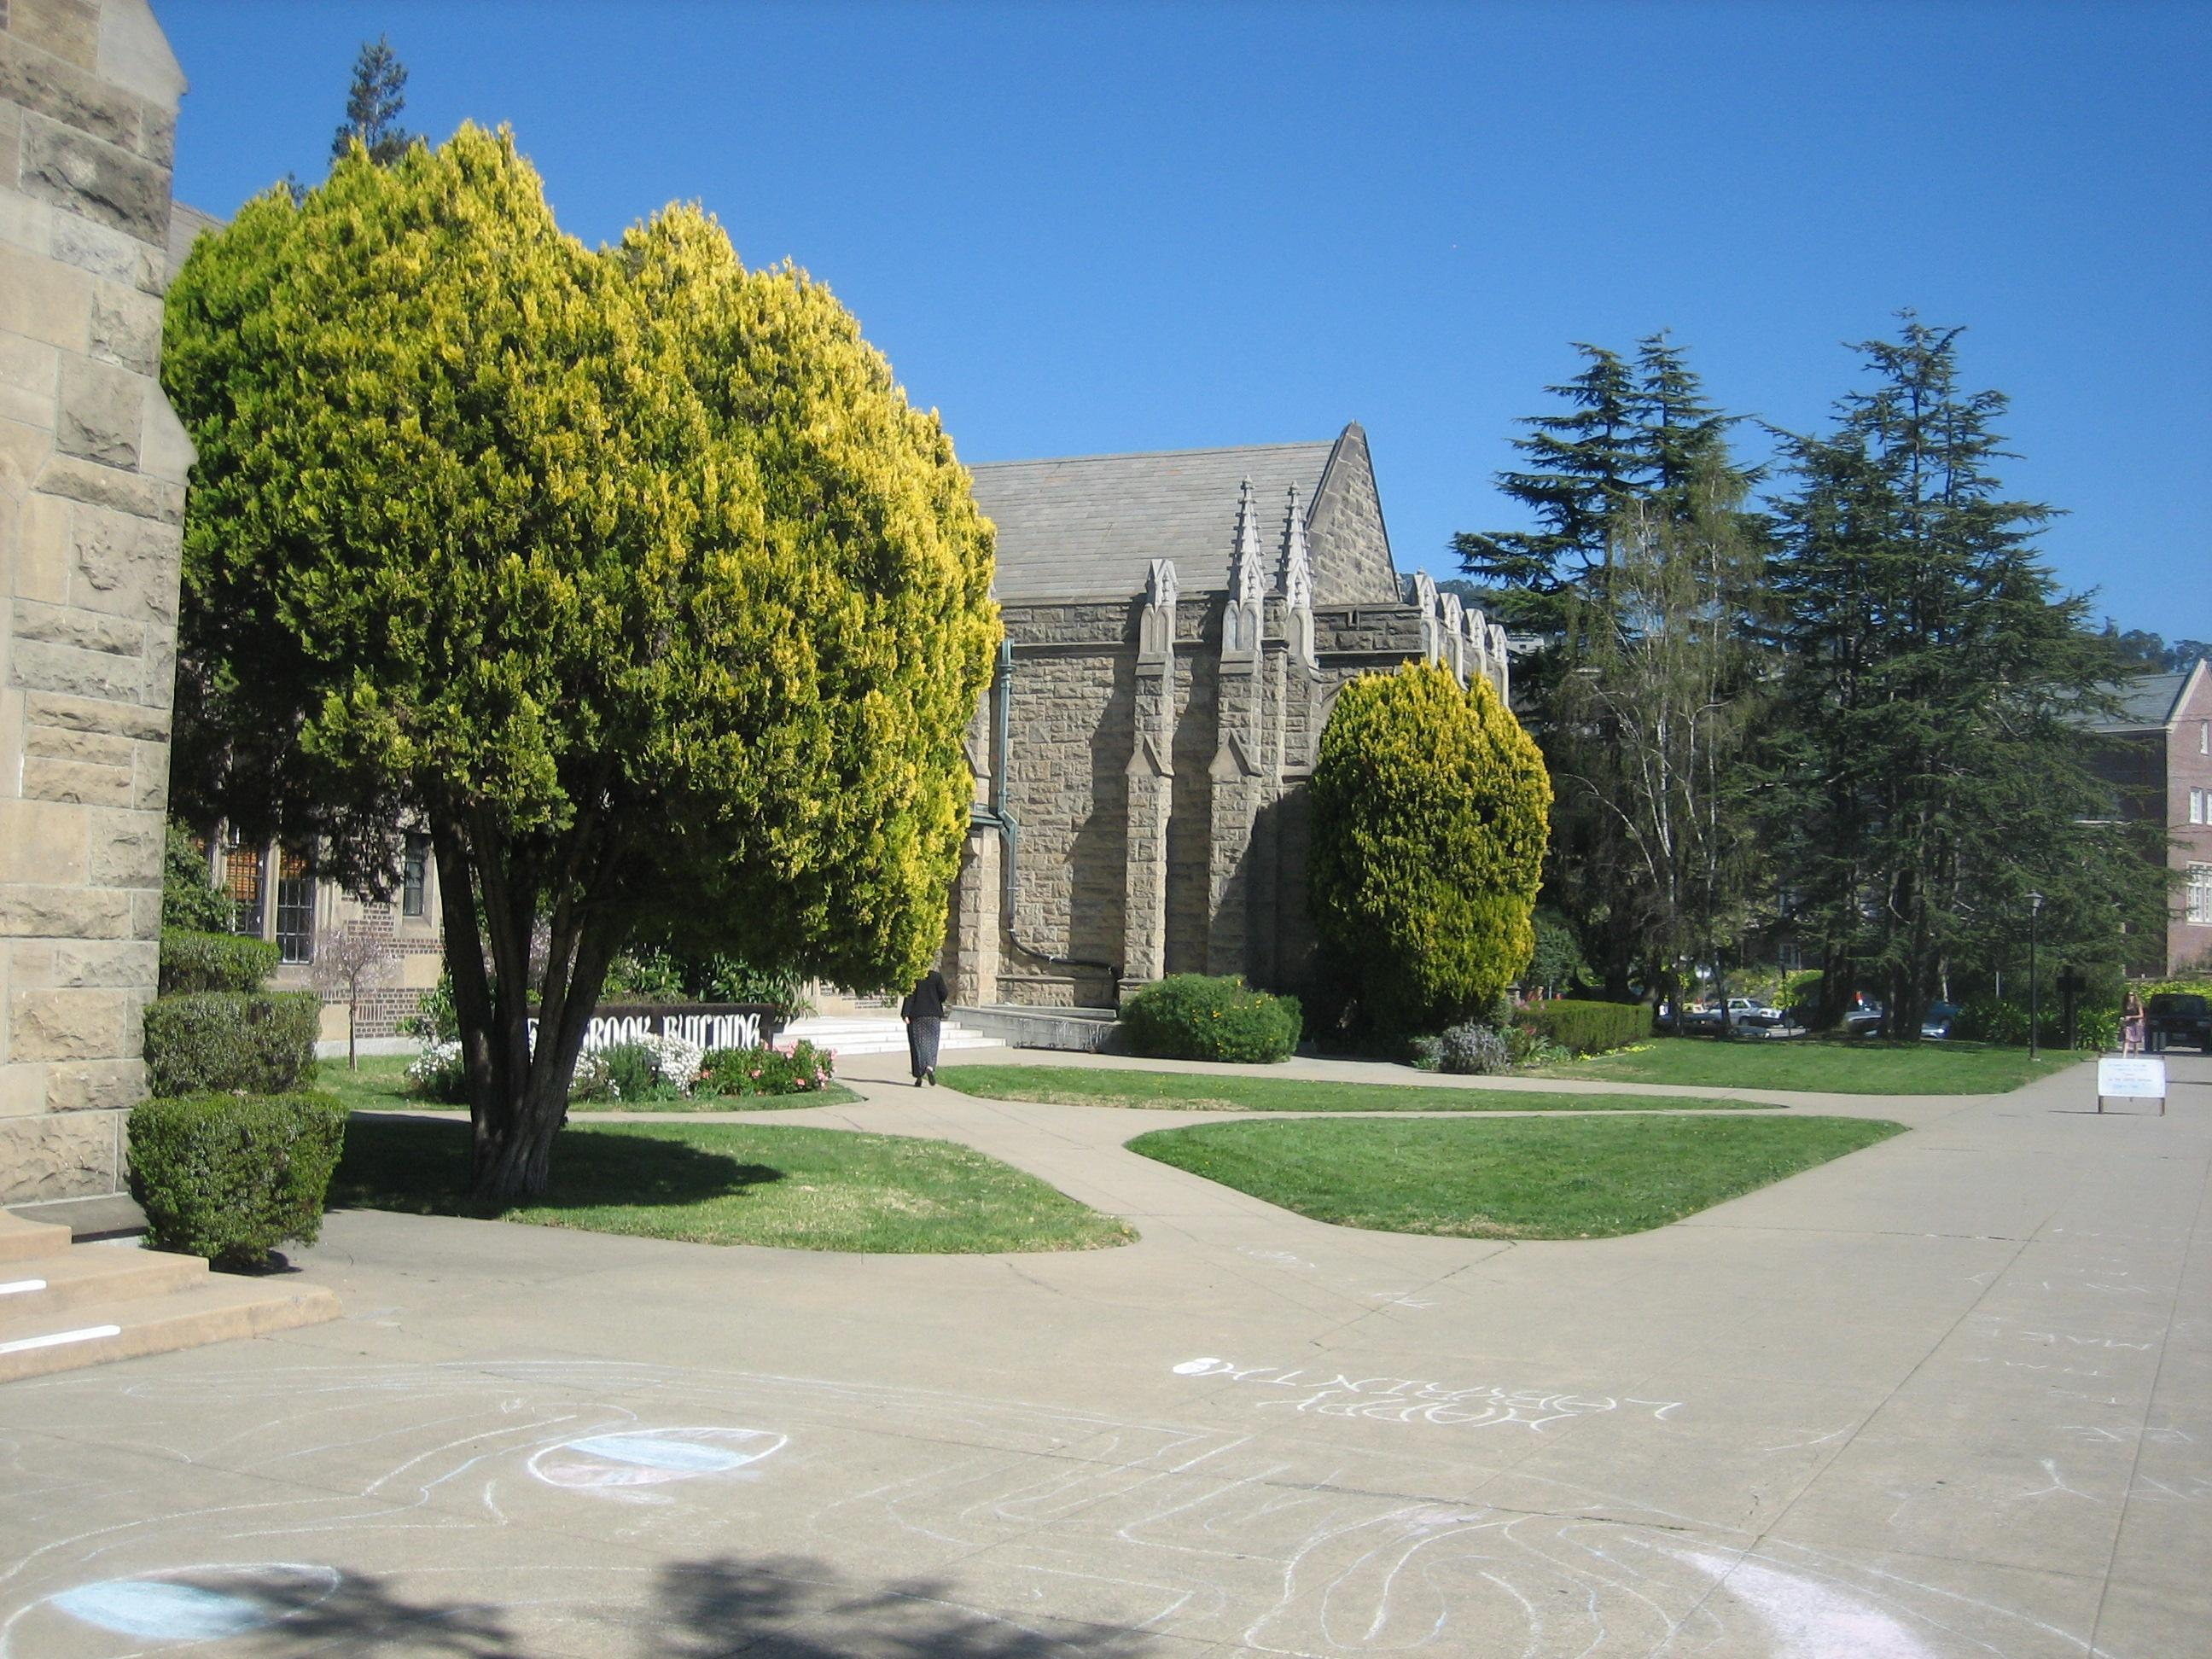
\includegraphics[width=4.0cm,height=4.0cm]{\input_image}};

\node[canvas is zy plane at x=0] (grid_yolo_130) at (image_yolo_130) {\drawgrid{4.0}{4.0}{0.25}};

\draw [connection] (conv_129-near) -- node {\midarrow} (yolo_130-far);

\pic[shift={(0, -3, 0)}] at (image_0.south)
    {RightBandedBox={
		name=legend_1,
		fill=\ConvColor,
		bandfill=\ConvReluColor,
		height=5.0,
		depth=5.0,
		width={1.0}
	}
};
\node [shift={(1,0,0)}, anchor=west] at (legend_1-east) {\LARGE{Convolution layer}};

\pic[shift={(0, -1, 0)}] at (legend_1-southwest)
{Box={
		name=legend_2,
		fill=\ShortcutColor,
		height=5.0,
		depth=5.0,
		width={1}
	}
};
\node [shift={(1,0,0)}, anchor=west] at (legend_2-east) {\LARGE{Shortcut layer}};

\pic[shift={(0, -1, 0)}] at (legend_2-southwest)
{Box={
		name=legend_3,
		fill=\DetectColor,
		height=5.0,
		depth=5.0,
		width={1}
	}
};
\node [shift={(1,0,0)}, anchor=west] at (legend_3-east) {\LARGE{Detection layer}};

\pic[shift={(0, -1, 0)}] at (legend_3-southwest)
{Box={
		name=legend_4,
		fill=\UpsampleColor,
		height=5.0,
		depth=5.0,
		width={1}
	}
};
\node [shift={(1,0,0)}, anchor=west] at (legend_4-east) {\LARGE{Upsample layer}};

\pic[shift={(0,-1,0)}] at (legend_4-south)
{Ball={
		name=legend_5,
		caption=,
		fill=\ConcColor,
		opacity=0.5,
		radius=2,
		logo=$\oplus$
	}
};
\node [shift={(0.75,0,0)}, anchor=west] at (legend_5-east) {\LARGE{Concatenation}};

\node[draw=black,ultra thick,inner sep=2ex,circle] (circle) at (yolo_83-anchor) {};
\node[shift={(2.5,-5,0)}](image_yolo) at (circle) {\scalebox{-1}[1]{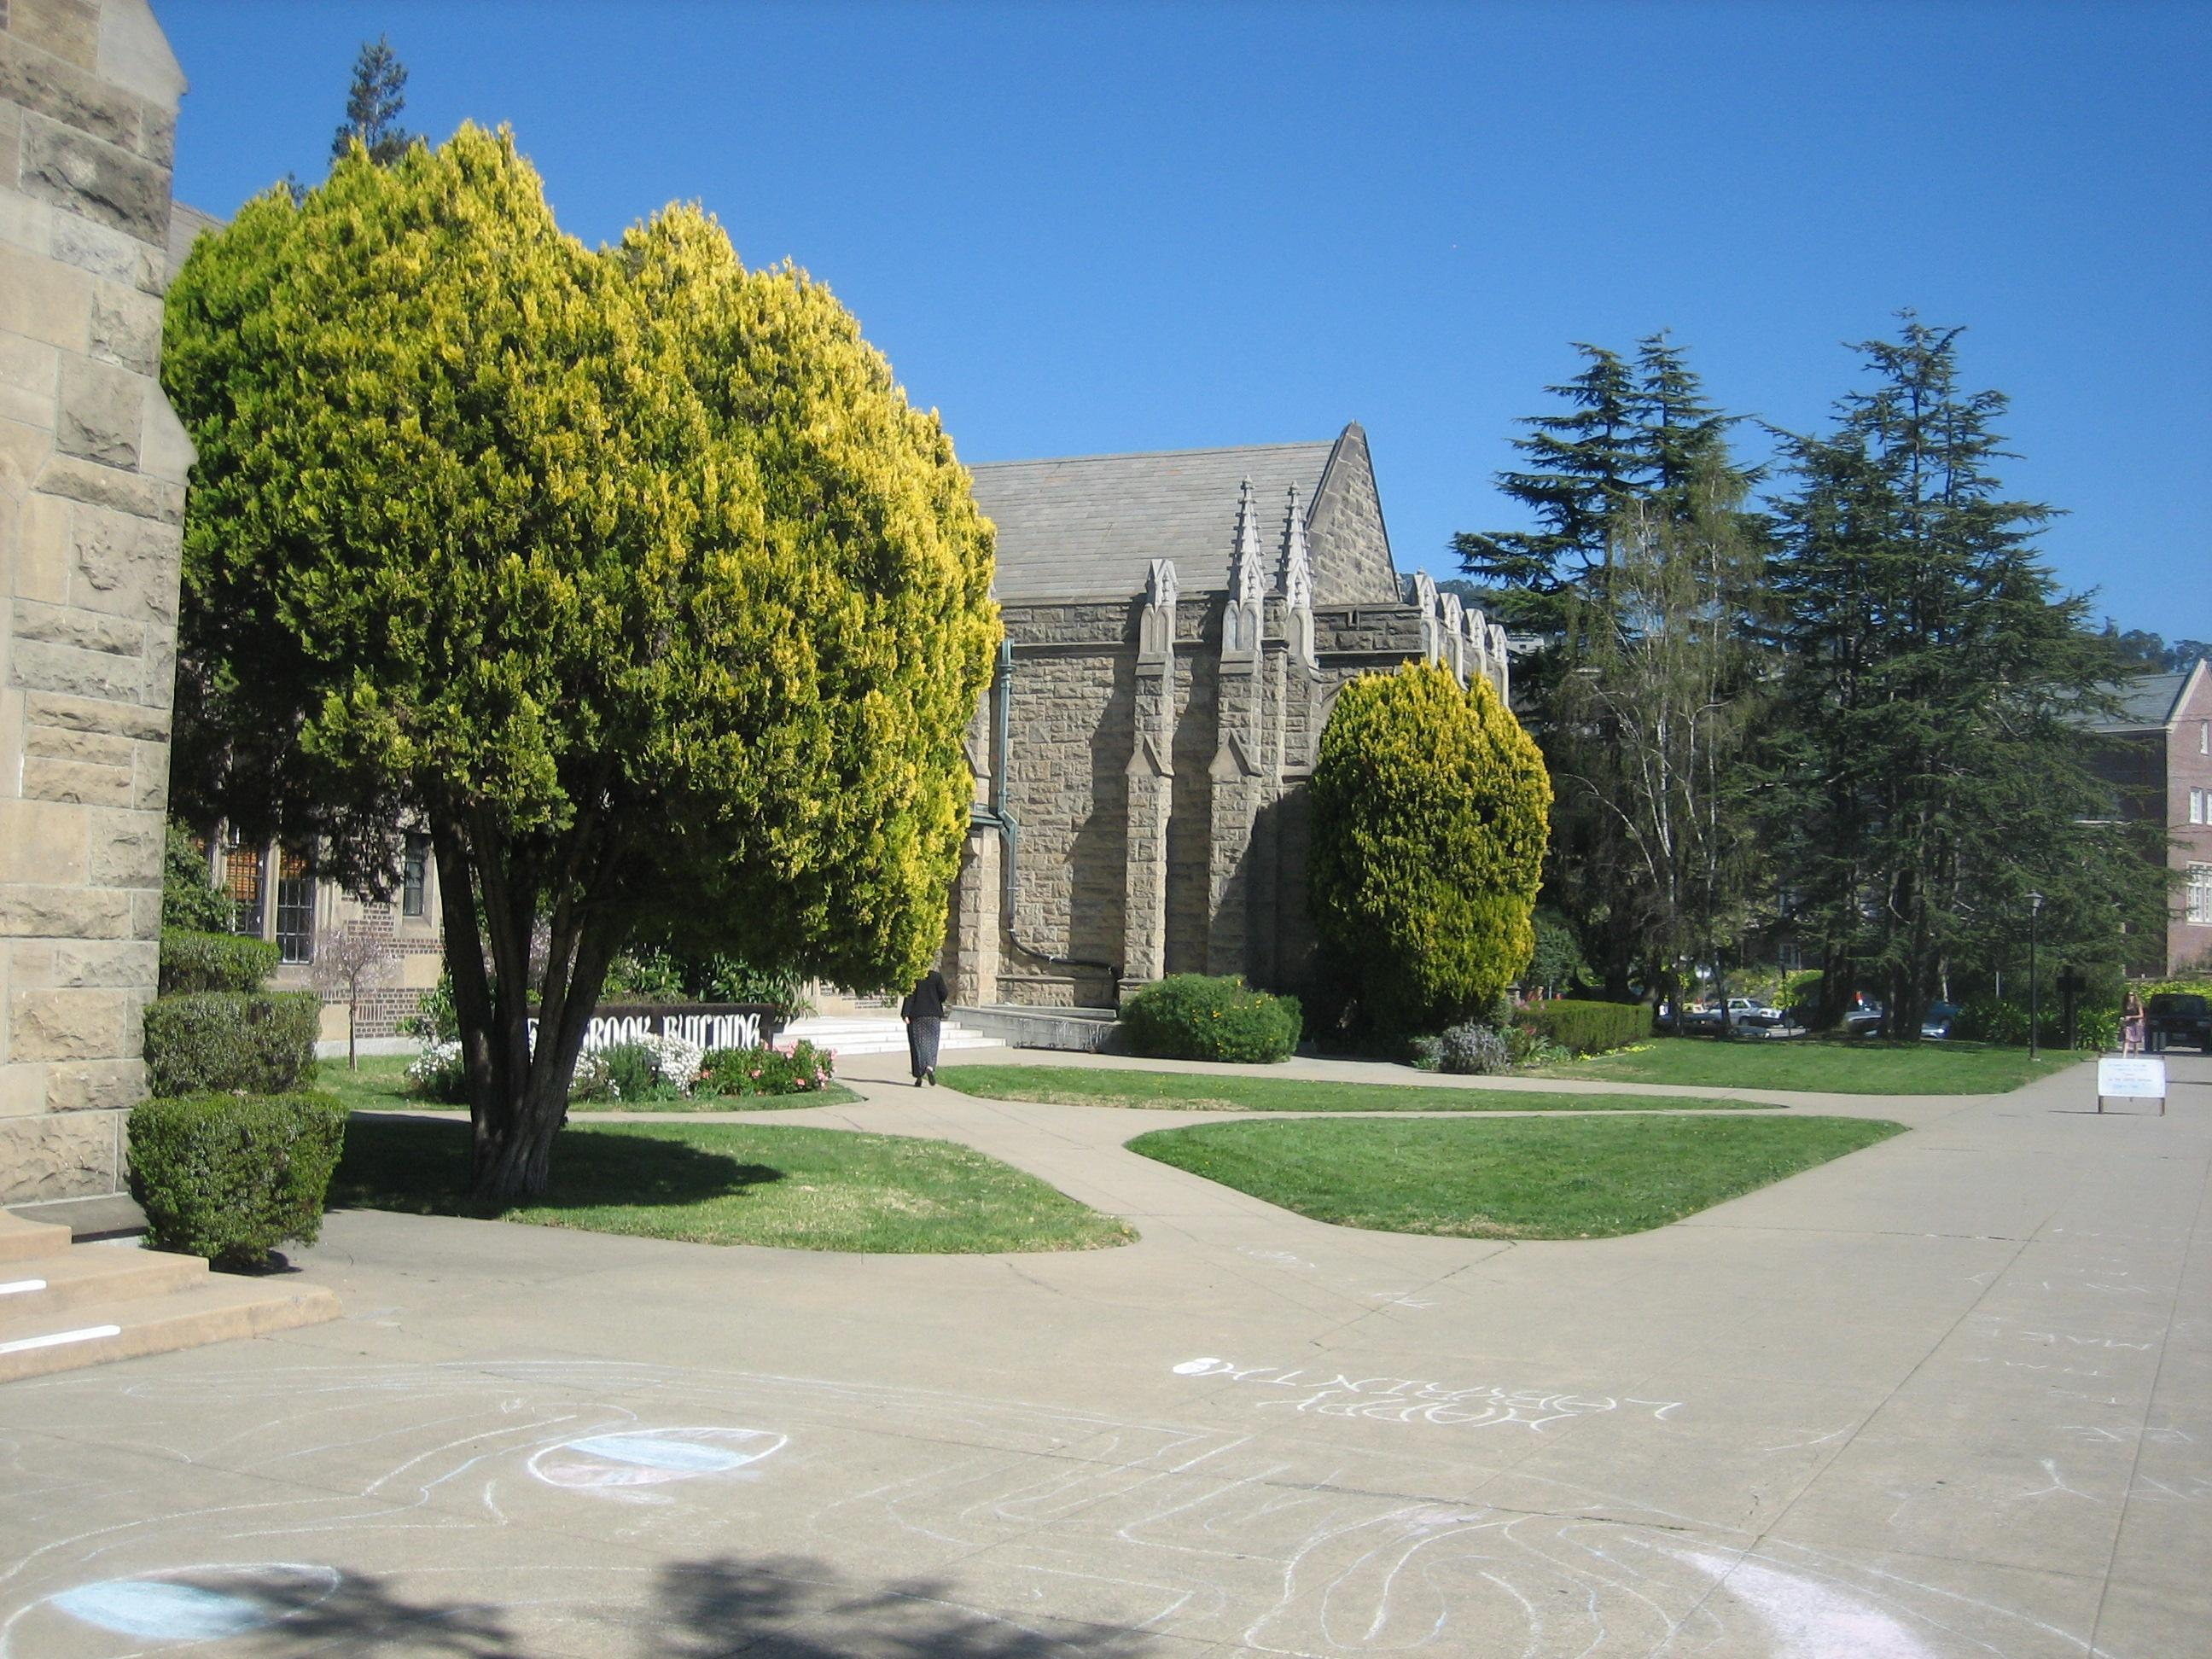
\includegraphics[width=5cm,height=5cm]{\input_image}}};
\node(grid_yolo_1) at (image_yolo) {\drawgrid{5}{5}{0.384615385}};
\node[canvas is zy plane at x=0] (grid_yolo_1) at (image_yolo_83) {\drawgrid{0.25}{0.25}{1.0}};
\node[draw=black,ultra thick,inner sep=2.5cm,rectangle] (rectangle) at (image_yolo) {};
\draw[ultra thick] (circle.south east) -- (rectangle.north);
\end{tikzpicture}

\end{document}
